\documentclass[10pt,a4paper]{article}
\usepackage[utf8]{inputenc}
\usepackage[czech]{babel}
\usepackage[T1]{fontenc}
\usepackage{graphicx}
\usepackage{amsmath}
\usepackage{ amssymb }
\usepackage{float}
\usepackage{fullpage}
\usepackage{color}
\usepackage{amsthm}
%\usepackage{vaucanson-g}				% makro pro kreslení grafů a automatů
\usepackage{alltt}


\setlength{\parindent}{0pt}
\setlength{\parskip}{1ex plus 0.5ex minus 0.2ex}

\newtheoremstyle{note}
{15pt}
{15pt}
{}
{}
{\bfseries}
{:}
{.5em}
{}
\theoremstyle{note}
\newtheorem{veta}{Věta}
\newtheorem{definice}{Definice}
\newtheorem{priklad}{Příklad}
\newtheorem{poznamka}{Poznámka}
\newtheorem{dusledek}{Důsledek}



\title{Teoretické základy informatiky}

\begin{document}
\maketitle

\newpage
\tableofcontents


\newpage

\section{První odstavec}

Formální jazyky a jejich hierarchie. Regulární jazyky (definice, uzávěrové vlastnosti). Konečné automaty deterministické
a nedeterministické. Regulární výrazy, automaty s epsilon-přechody. Minimalizace konečného deterministického
automatu. Pumping lemma. Bezkontextové jazyky a jejich vlastnosti (uzávěrové vlastnosti, jednoznačnost).
Zásobníkové automaty a jejich modifikace. Deterministické zásobníkové automaty. Deterministické
bezkontextové jazyky.

	\subsection{Formální jazyky a jejich hierarchie}

		Zaveďme si pojem \textit{formální jazyk nad množinou všech řetězců} $\Sigma^{*}$. Označme tento jazyk jako $L$. 				Pak platí tato tvrzení:
		\begin{eqnarray*}
			L &\subseteq& \Sigma^{*} \text{ (každá podmnožina abecedy je jazykem)} \\
			L &=& \emptyset \text{ (prázdný jazyk)} \\
			L &=& \lbrace \varepsilon \rbrace \text{ (jazyk s prázdným řetězcem)} \\
			&\vdots&
		\end{eqnarray*}
		\textit{Pozor, obecně platí že prázdný jazyk $\neq$ jazyk s prázdným řetězcem.}

		Formálním jazykem obecně myslíme nějakou množinu \textit{řetězců}, které navíc většinou mají určitou
		společnou vlastnost, jak uvidíme později.

		\subsubsection{Operace nad jazyky}

		\subsubsection{Množinové}
		Množinové operace nad jazyky jsou prakticky totožné operacím na kterýchkoliv jiných množinách.
		Můžeme tedy použít množinový průnik, sjednocení, komplement (doplněk) nebo rozdíl.

		\subsubsection{Ostatní}
		\begin{itemize}
		\item
		\textit{Zřetězení} (produkt) množin. Vyjádřeme produkt takto:
		$$
		L_{1}L_{2} = \lbrace xy | x \in L_{1}, y \in L_{2} \rbrace
		$$
		Produkt množin není obecně komutativní, ale je asociativní, přičemž prázdná množina tuto operaci anihiluje.
		Uveďme si rovněž monoid $\langle 2^{\Sigma^{*}}, \circ, \lbrace \varepsilon \rbrace \rangle$.

		\item
		\textit{}{Mocnina} jazyka. Mocninu vyjádříme takto:
		$$
		L^{n} = \left \lbrace
		\begin{array}{l l}
		\lbrace \varepsilon \rbrace & \text{ pro } n = 0 \\
		LL^{n-1} & \text{ pro } n \geq 1 \\
		\end{array}
		\right.
		$$

		\item
		\textit{Kleeneho} uzávěr neboli 	\textit{iterace}. Tento uzávěr vyjádříme takto:
		$$
		L^{*} = \bigcup_{i = 0}^{\infty} L^{i}
		$$

		\item
		\textit{Pozitivní} uzávěr neboli pozitivní iterace. Tento uzávěr vyjádříme takto:
		$$
		L^{+} = \bigcup_{i = 1}^{\infty} L^{i}
		$$
		Všimněte si podobností mezi těmito dvěma uzávěry. Pozitivní uzávěr vynechává prázdný řetězec.

		\end{itemize}

		\textbf{GRAMATIKY}\\

		\vspace{3mm}
		Jak víme, tak jazyky mohou být \textit{nekonečné} ve smyslu, že obsahují nekonečný počet slov.
		Nabízí se tedy otázka, jak tyto jazyky rozumně popsat, jak je reprezentovat resp. jak vytvořit \textit{konečnou}
		sadu pravidel, jejichž aplikace by vedla k opětovné generaci původního jazyka.


		\textbf{Přepisovací pravidla}\\

		\vspace{3mm}
		Pravidlem rozumíme zpravidla každou dvojici:
		$$
		\langle x,y \rangle \in \Sigma^{*} \times \Sigma^{*}
		$$
		Pak neformálně tvrdíme, že $x$ \textit{se přepisuje} na $y$.
		Nutno dodat, že předchozí zápis lze zapsat i například takto.
		$$
		x \rightarrow y\text{, kde symbol } \rightarrow \notin \Sigma \text{ můžeme prohlásit za tzv. metasymbol.}
		$$
		\textbf{Vlastnosti pravidel}\\

		\vspace{3mm}
		\begin{itemize}
		\item \textit{Nezkracující} pravidlo je pravidlo, o kterém platí, že $|x| \leq |y|$. Tedy aplikaci tohoto pravidla
		 na vstupní řetězec určitě nevznikne řetězec kratší, než-li jeho předloha.

		\item $\varepsilon$ - pravidlo je pravidlo tvaru $x \rightarrow \varepsilon$.
		\end{itemize}


		\textbf{Příklady pravidel}\\

		\vspace{3mm}
		\begin{priklad}
		Mějme zadání abecedy $\Sigma = \lbrace a,b,c \rbrace$. Pravidla s využitím této abecedy by mohla být například tato.
		\begin{eqnarray*}
		aa &\rightarrow& bc \\
		bb &\rightarrow& abba \\
		c &\rightarrow& \varepsilon
		\end{eqnarray*}
		\end{priklad}

		\begin{priklad}
		Mějme další zadání abecedy $\Sigma = \lbrace expr, +, \times \rbrace$. Pravidla s využitím této abecedy by 
		mohla být například takto.
		\begin{eqnarray*}
		\textit{expr} &\rightarrow& \textit{expr} + \textit{expr} \\
		\textit{expr} &\rightarrow& \textit{expr} \times \textit{expr}
		\end{eqnarray*}
		\end{priklad}


		\textbf{Přímé odvozování řetězců pomocí pravidel}\\

		\vspace{3mm}
		Uvažujme odvozovací pravidlo $ x \rightarrow y \text{ nad abecedou } \Sigma$, pak řekneme,
		 že řetězec \textit{v} \textit{je přímo odvozen}
		z řetězce \textit{u} pomocí pravidla $ x \rightarrow y $, pokud $\exists p, q \in \Sigma^{*}$ tak, že
		\begin{gather*}
		u = p x q \\
		v = p y q
		\end{gather*}

		Značení předchozí operace je následující:
		$$
		u \Rightarrow_{x \rightarrow y} v
		$$
		Slovně bychom tento zápis vystihli jako \uv{přímý přepis dle pravidla $x \rightarrow y$.}

		Řetězec $v$ vznikne přímým přepisem z $u$ pomocí pravidel $P \subseteq  \Sigma^{*} \times \Sigma^{*}$, pokud
		$\exists \pi \in P \text{ tak, že } u \Rightarrow_{\pi} v$.

		Značme $u \Rightarrow_{P} v$. $P$ je množinou užitých pravidel. $P$ i $\Rightarrow_{p}$ jsou binární relace
		 na 	$\Sigma^{*}$ a
		$P \subseteq  \Rightarrow_{p}$, tedy \uv{P je podmnožinou šipky p.} Platí, že $x \rightarrow y \in P$
 		a $x \Rightarrow_{x \rightarrow y} y$.
		Můžeme tedy poněkud nadneseně říci, že množina pravidel $P$ obsahuje jen podmnožinu všech možných pravidel,
		 který je možno sestrojit
		nad danými terminálními a neterminálními symboly (o těch se dozvíme více informaci později).

		\begin{priklad}
		Mějme abecedu $\Sigma = \lbrace a, b, c \rbrace$ a soubor pravidel $P = \lbrace aa \rightarrow bc, a
		 \rightarrow cab, bb \rightarrow \varepsilon \rbrace$\label{priklad-1}.
		Pak by odvození v jednom kroku mohla vypadat například takto:
		\begin{gather*}
		baaa \rightarrow bbca \\
		bac \rightarrow bcabc
		\end{gather*}
		\end{priklad}

\begin{definice}
Definujme pojem \textit{derivace}. Jedná se o posloupnost řetězců ve tvaru:
$$
x_{0}, \ldots, x_{k},\text{ kde } k \geq 0\text{ a kde } \lbrace x_{0}, \ldots, x_{k} \rbrace \in \Sigma^{*}
$$
se nazývá \textit{P-derivace délky k}, pokud $x_{i-1} \Rightarrow_{p} x_{i}, \forall 1 \leq i \leq k $.
Symbolicky totéž $x_{0} \Rightarrow_{p} x_{1} \Rightarrow_{p} \ldots \Rightarrow_{p} x_{k}$. Počet odvození tedy značí \textit{délku} derivace.
\end{definice}

Pokud pro $u, v \in \Sigma^{*} \quad \exists \text{ P-derivace } u = x_{0} \ldots x_{k} = v$, pak říkáme, že $v$ je odvozeno z $u$ pomocí pravidel z $P$, což značíme
například $u \Rightarrow_{P}^{*} v$, tímto je pochopitelně myšleno odvození ve více krocích. Platí, že $P \subseteq \Rightarrow_{P} \subseteq \Rightarrow_{P}^{+}$.

\begin{priklad}
Mějme abecedu $\Sigma = \lbrace a, \ldots, z \rbrace$ a pravidla stejná jako v příkladu \ref{priklad-1}.
Nyní odvozujeme například takto:
$$
b\underline{aa}a, \underline{bb}ca, c\underline{a}, c\underline{cab}
$$
\end{priklad}

\textbf{Formální gramatiky}\\

		\vspace{3mm}
Mějme následující entity:
\begin{itemize}
\item $\Sigma$ - abeceda terminálních symbolů (tyto symboly tvoří řetězce daného jazyka).
\item $N$ - abeceda neterminálních symbolů (tyto symboly se užívají k řízení průběhu odvozování).
\end{itemize}

Dodejme, že obě množiny by měly být neprázdné a konečné.

\begin{definice}
Odvozovací pravidlo $x \rightarrow y$ se nazývá \textit{generativní}, pokud \textit{x} obsahuje alespoň jeden neterminální symbol.
\end{definice}

\begin{definice}
Mějme strukturu $G = \langle N, \Sigma, P, S \rangle$, kde $N$ je abecedou neterminálních symbolů, $\Sigma$ je abecedou terminálních symbolů,
$P$ je množinou odvozovacích pravidel a $S \in N$ je tzv. \textit{počátečním} resp. \textit{startovním} neterminálem. Pak tuto čtveřici nazveme \textit{gramatikou}.
\end{definice}

\begin{poznamka}
Pokud chceme vyjádřit, že z jednoho symbolu odvozujeme několik možných alternativ, tak to zapíšeme místo klasického dlouhé zápisu
$y \rightarrow x_{1}, y \rightarrow x_{2}, \ldots$ pomocí zkrácené notace např. $y \rightarrow x_{1}|x_{2}|\ldots$
\end{poznamka}

\begin{priklad}
Gramatika může vypadat třeba takto:
\begin{eqnarray*}
N &=& \lbrace \varepsilon, S, D, I \rbrace \\
\Sigma &=& \lbrace 0, \ldots, 9, +, - \rbrace \\
P &=& \lbrace S \rightarrow -I|+I|I, I \rightarrow DI|D, D \rightarrow 0|1|\ldots |9 \rbrace \\
G &=& \langle N, \Sigma, P, S \rangle
\end{eqnarray*}
\end{priklad}

\begin{priklad}\label{priklad-2}
Nebo takto:
\begin{eqnarray*}
N &=& \lbrace S, X, Y \rbrace \\
\Sigma &=& \lbrace a, b, c \rbrace \\
P &=& \lbrace S \rightarrow XcYcX, X \rightarrow aX, X \rightarrow bX, X \rightarrow cX, X \rightarrow \varepsilon,
Y \rightarrow abY, Y \rightarrow ab \rbrace \\
G &=& \langle N, \Sigma, P, S \rangle
\end{eqnarray*}
\end{priklad}

\begin{definice}
Každý řetězec $x \in (N \cup\Sigma)^{*}$, pro který platí $S \rightarrow^{*} x$, je \textit{větná forma} gramatiky $G = \langle N, \Sigma, P, S \rangle$.
Větná forma se nazývá \textit{větou}, pokud $x \in \Sigma^{*}$.
\end{definice}

\begin{definice}
Jazyk generovaný gramatikou definujme jako:
$$
L(G) = \lbrace x \in \Sigma^{*} | S \Rightarrow_{G}^{*} x \rbrace
$$
Vidíme tedy, že takový jazyk obsahuje \textit{věty}, které lze odvodit ze startovacího neterminálu pomocí pravidel této gramatiky.
\end{definice}

\begin{priklad}
Tento příklad čerpá gramatiku z příkladu \ref{priklad-2}.
\begin{eqnarray*}
S &\Rightarrow_{G}^{*}& abbccYcX \\
S &\Rightarrow_{G}^{*}& Xcababababc \\
S &\Rightarrow_{G}^{*}& cYcbaX \\
S &\Rightarrow_{G}^{*}& abbccabca \\
S &\Rightarrow_{G}^{*}& cabababc
\end{eqnarray*}
\end{priklad}

\begin{definice}
Gramatiky $G_{1}$ a $G_{2}$ jsou \textit{ekvivalentní}, pokud generují stejný jazyk.
\end{definice}

\subsubsection{Hierarchie gramatik}
\begin{itemize}
\item
\textit{Gramatiky typu 0} -- jedná se o gramatiky bez omezení.

\item
\textit{Gramatiky typu 1\label{gram-1}} -- jedná se o tzv. \textit{kontextové} nebo \textit{kontextově závislé} gramatiky.
Ty splňují následující omezení na tvar pravidel. Pro každé pravidlo gramatik tohoto typu platí, že:
\begin{enumerate}
\item
Buď je (pravidlo) ve tvaru $pAq \rightarrow p x q, \text{ kde } p, q \in (\Sigma \cup N)^{*}, A \in N, x \in (\Sigma \cup N)^{+}$, kde \textit{p} a \textit{q}
se nazývají levým resp. pravým \textit{kontextem}.

\item
Nebo je (pravidlo) ve tvaru $S \rightarrow \varepsilon$, kde $S$ je startovní terminál gramatiky, ale pouze
za předpokladu, že $S$ se nevyskytuje na pravé straně žádného pravidla.
\end{enumerate}

Zároveň platí pro každé pravidlo (s výjimkou pravidla $S \rightarrow \varepsilon$), že délka odvozeného řetězce je minimálně stejně velká jako délka vstupního řetězce. Gramatika tedy zároveň obsahuje pouze tzv. \textit{nezkracující} pravidla.

\item
\textit{Gramatiky typu 2} -- jedná se o tzv. \textit{bezkontextové} gramatiky, jenž obsahují pravidla ve tvaru:
$$
A \rightarrow x, \text{ kde } A \in N, x \in (\Sigma \cup N)^{+}
$$
Na levých stranách pravidel tedy očekáváme pouze neterminální symbol a na pravé straně očekáváme minimálně jeden symbol (s výjimkou $\varepsilon$-pravidla).

Očividně platí, že je-li gramatika bezkontextová, pak je i kontextová, nebo $p=\varepsilon, q=\varepsilon$ jsou také kontexty, byť jsou \uv{prázdné}.

\begin{priklad}
Mějme tuto gramatiku:
\begin{eqnarray*}
G &=& \langle N, \Sigma, P, S \rangle \\
N &=& \lbrace A, S \rbrace \\
\Sigma &=& \lbrace 0, 1 \rbrace \\
P &=& \lbrace S \rightarrow 0A, A \rightarrow \varepsilon \rbrace
\end{eqnarray*}
\end{priklad}

\item
\textit{Gramatiky typu 3\label{gram-3}} -- jedná se o tzv. \textit{regulární} resp. \textit{pravolineární} gramatiky, které obsahují pravidla ve třech následujících tvarech:

\begin{enumerate}
\item
$A \rightarrow bB, \text{ kde } A,B \in N, b \in \Sigma$

\item
$A \rightarrow a$

\item
$S \rightarrow \varepsilon$ (přičemž platí stejné podmínky, jako u gramatik typu 1)
\end{enumerate}

\end{itemize}

\begin{veta}
Každý konečný jazyk je regulární.
\end{veta}


\begin{figure}[ht]
\centering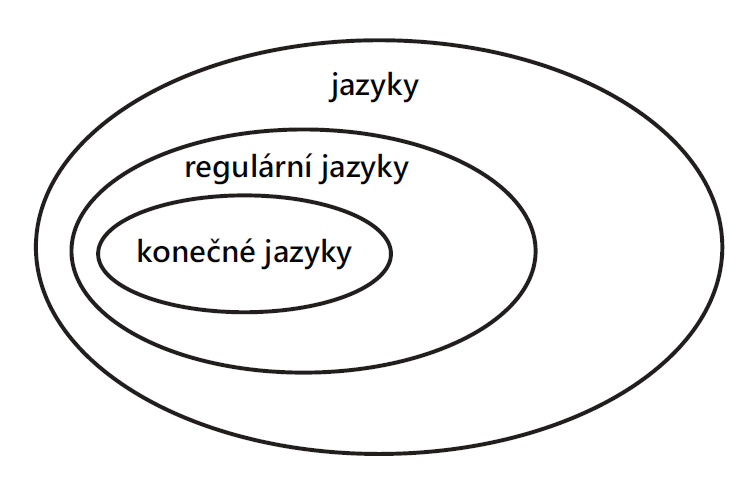
\includegraphics[width=8cm]{img/vychodilovoVajicko}
\caption{Vychodilovo \uv{vajíčko.}}\label{obr-2}
\end{figure}

\vspace{30px}

\begin{priklad}
\begin{eqnarray*}
N &=& \lbrace S \rbrace \\
\Sigma &=& \lbrace a, b \rbrace \\
P &=& \lbrace S \rightarrow aSb | \varepsilon \rbrace \\
L(G) &=& \lbrace a^{n}b^{n} | \quad n \geq 0 \rbrace
\end{eqnarray*}
Máme tedy \textit{bezkontextový} jazyk.
\end{priklad}

\begin{priklad}
\begin{eqnarray*}
N &=& \lbrace S \rbrace \\
\Sigma &=& \lbrace a, b \rbrace \\
P &=& \lbrace S \rightarrow SS|aSb|bSa| \varepsilon \rbrace
\end{eqnarray*}
$L(G)$ je \textit{bezkontextový} jazyk.
\end{priklad}

\begin{priklad}
\begin{eqnarray*}
N &=& \lbrace S, V \rbrace \\
\Sigma &=& \lbrace p,),(, \Rightarrow, ! \rbrace \\
P &=& \lbrace S \rightarrow V|(S \Rightarrow S)|!S, V \Rightarrow pV|p \rbrace
\end{eqnarray*}
$L(G)$ je jazyk všech výrokových formulí.
\end{priklad}


%----------------------------------------------------------------------------------------------------------------------
	\subsection{Regulární jazyky (definice, uzávěrové vlastnosti)}

		\textit{Gramatiky typu 3} -- jedná se o tzv. \textit{regulární} resp. \textit{pravolineární} gramatiky, které obsahují pravidla ve třech následujících tvarech:

\begin{enumerate}
\item
$A \rightarrow bB, \text{ kde } A,B \in N, b \in \Sigma$

\item
$A \rightarrow a$

\item
$S \rightarrow \varepsilon$ (přičemž platí stejné podmínky, jako u gramatik typu 1)
\end{enumerate}


\begin{veta}
Každý konečný jazyk je regulární.
\end{veta}

\subsubsection{Vztah regulárních jazyků a konečných automatů}

\paragraph{Regulární jazyky jsou rozpoznatelné KDA (implikace zleva)}

\begin{veta}
Pro každou regulární gramatiku $G=\langle N,\Sigma,P,S \rangle$ existuje konečný deterministický automat $A$ tak, že jazyk generovaný gramatikou je totéž, jako jazyk rozpoznatelný automatem, tj. $L(G)=L(A)$
\end{veta} 



V případě, že $\varepsilon \in L(G)$, rozšíříme automat následovně, jednou ze tří možností:
\begin{enumerate}
\item
Přidáme $S$ do množiny koncových stavů.

\item
Přidáme $\#$ mezi počáteční stavy.\footnote{Též nazývána jako \uv{Konyho finta}.}

\item
Zavedeme nový stav, který bude počáteční a zároveň koncový a nevedou z něj žádné přechody jinam.
\end{enumerate}

\begin{poznamka}
Nyní zbývá automat pouze determinizovat.
\end{poznamka}

\begin{priklad}
Máme gramatiku $G$.
\begin{eqnarray*}
G &=& \langle N,\Sigma,P,S \rangle \\
\Sigma &=& \lbrace e,d,. \rbrace \\
P &=& \lbrace S \rightarrow .F | dT , T \rightarrow .E|.F|dT|. , D \rightarrow dD|d , E \rightarrow eD , F \rightarrow dE|dF|d \rbrace
\end{eqnarray*}

Automat rozpoznávající jazyk, generovaný gramatikou G, bude vypadat následovně:

\begin{center}
\centering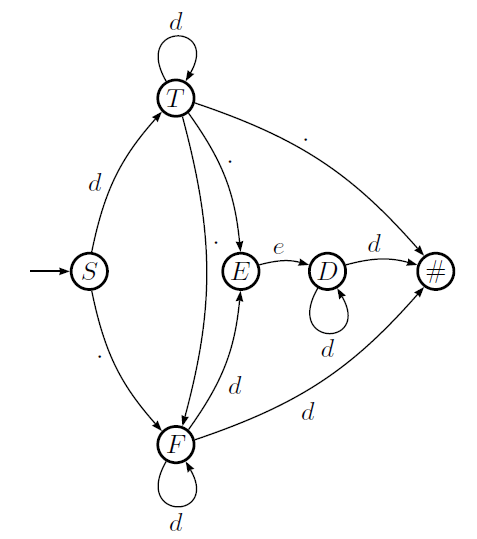
\includegraphics[width=8cm]{img/reg1}
\end{center}

Když tento automat zdeterminizujeme, dostaneme následující automat:

\begin{center}
\centering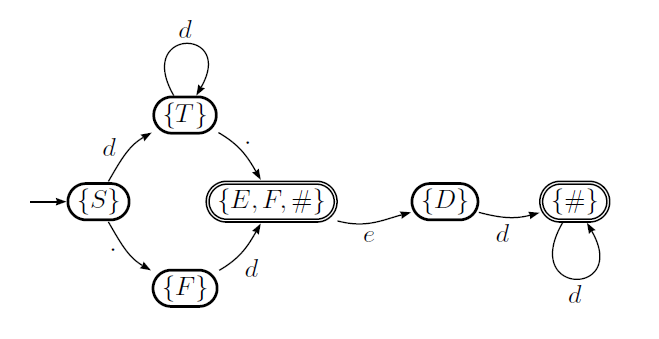
\includegraphics[width=8cm]{img/reg2}
\end{center}

\end{priklad}

\subsection{Jazyky rozpoznatelné KDA jsou regulární (implikace zprava)}

\begin{veta} 
Pro každý konečný deterministický automat $A = \langle \Sigma,Q,\delta,q_0,F \rangle$ existuje regulární gramatika $G$ tak, že $L(A)=L(G)$.
\end{veta}


\begin{priklad}\label{priklad-4}

Mějme abecedu $\Sigma = \lbrace a,b \rbrace$ a automat zadaný diagramem:
\begin{center}
\centering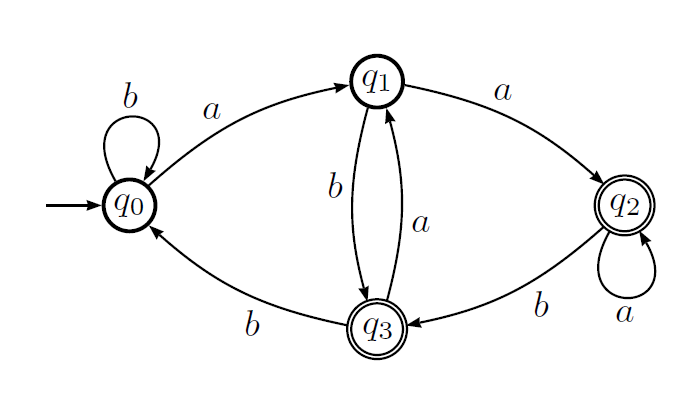
\includegraphics[width=8cm]{img/reg3}
\end{center}

Odvozovací pravidla gramatiky, generující tento jazyk budou:

\begin{eqnarray*}
q_0 &\rightarrow& aq_1\ |\ bq_0 \\
q_1 &\rightarrow& aq_2\ |\ a\ |\ bq_3\ |\  b \\
q_2 &\rightarrow& aq_2\ |\ a\ |\ bq_3\ |\  b \\
q_3 &\rightarrow& aq_1\ |\ bq_0
\end{eqnarray*}

\end{priklad}

\subsubsection{Regulární gramatiky}

Co jsou to regulární gramatiky a jaké podmínky jejich odvozovací pravidla splňují již víme, ale můžeme si je ještě rozdělit na dva druhy, právě podle tvaru odvozovacích pravidel.

\begin{enumerate}

\item
\textit{Zprava regulární gramatiky:}
Obsahují pravidla ve tvaru $ A \rightarrow bB $, tedy neterminál je napravo od terminálního symbolu.
\item
\textit{Zleva regulární gramatiky:}
Obsahují pravidla ve tvaru $ A \rightarrow Bb $. Analogicky se neterminál nachází vlevo od terminálního symbolu.
\end{enumerate}

\begin{veta}
Pro každou zleva regulární gramatiku $ G = \langle N,\Sigma,P,S \rangle $ existuje konečný deterministický automat \textit{A} tak, že \textit{L(A)=L(G)}.
\end{veta}


\begin{priklad}
Máme gramatiku $G$ s následovně definovanými pravidly.
\begin{eqnarray*}
S &\rightarrow& Aa|Ba|Bb|a \\
A &\rightarrow& Aa|Bb \\
B &\rightarrow& Ab|Ba|b
\end{eqnarray*}

Automat rozpoznávající jazyk generovaný touto gramatikou bude vypadat následovně:

\begin{center}
\centering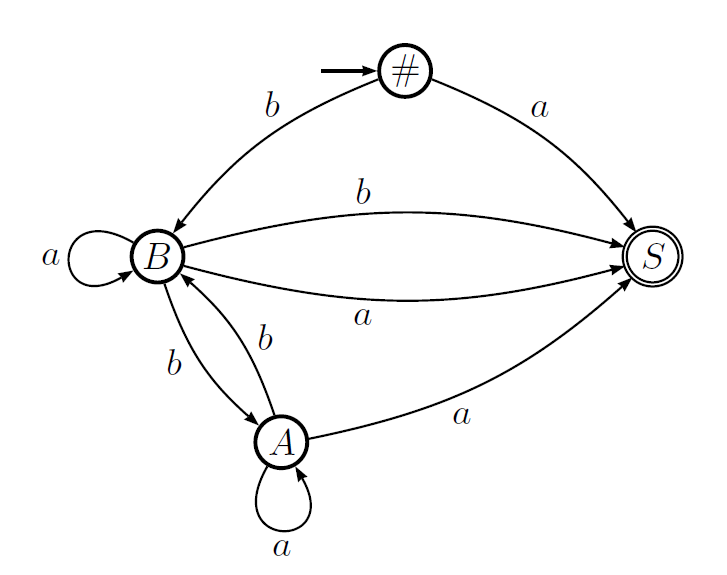
\includegraphics[width=8cm]{img/reg4}
\end{center}

\end{priklad}

\begin{veta}
Pro každý konečný deterministický automat \textit{A} existuje zleva regulární gramatika taková, že \textit{L(A)=L(G)}
\end{veta}


\begin{priklad}
Vezmeme KDA z příkladu 
Odvozovací pravidla budou vypadat takto:

\begin{eqnarray*}
q_0 &\rightarrow& q_{0}b\ |\ b\ |\ q_{3}b \\
q_1 &\rightarrow& q_{0}a\ |\ a\ |\ q_{3}a \\
q_2 &\rightarrow& q_{1}a\ |\ q_{2}a \\
q_3 &\rightarrow& q_{1}b\ |\ q_{2}b \\
S &\rightarrow& q_{1}a\ |\ q_{1}b\ |\ q_{2}a\ |\ q_{2}b \\
\end{eqnarray*}

\end{priklad}

\begin{definice}
Regulární jazyky jsou jazyky, generované zprava (zleva) regulárními gramatikami, tj. jsou rozpoznatelné konečnými ne/deterministickými automaty.
\end{definice}

\begin{poznamka}
Pravidla zprava a zleva nelze míchat.
\end{poznamka}





\subsubsection{Uzávěrové vlastnosti regulárních jazyků}

\paragraph{Základní uzávěrové vlastnosti}

\begin{itemize}
\item
\textit{Komplement}

Pokud je $L$ regulární, pak je $\Sigma^* \backslash L$ regulární.


\item
\textit{Sjednocení} 

Jsou-li $L_1$ a $L_2$ regulární, pak je $L_1 \cup L_2$ regulární.


\begin{priklad}
Nyní si uvedeme protipříklad, co by se stalo, kdyby množiny stavů nebyly disjunktní.

\begin{figure}[H]
\centering
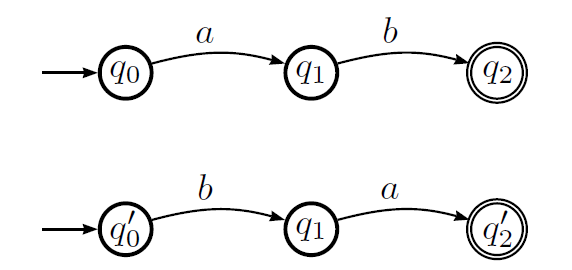
\includegraphics[width=8cm]{img/reg5}
\end{figure}

První automat přijímá řetězec $ab$, druhý automat přijímá řetězec $ba$, čili od jejich sjednocení očekáváme, že bude přijímat $ab$ i $ba$. Jelikož množiny stavů nejsou disjunktní ($q_1$ je společný pro oba), sjednocení těchto automatů může stejně dobře přijímat i řetězce $aa$ nebo $bb$, což je nežádoucí.
\end{priklad}

\item
\textit{Průnik} 

S použitím De Morganových zákonů, dostáváme:
$$L_1 \cap L_2 = \Sigma^* \backslash (\Sigma^* \backslash L_1 \cup \Sigma^* \backslash L_2 )$$
tj. $L_1 \cap L_2$ je regulární.


\item
\textit{Produkt (zřetězení)} 

$L_1 \cdot L_2$

Předpokládáme existenci automatů $A_1$ a $A_2$ takových, že $L_1 = L(A_1)$ a $L_2 = L(A_2) $.

\begin{figure}[H]
\centering
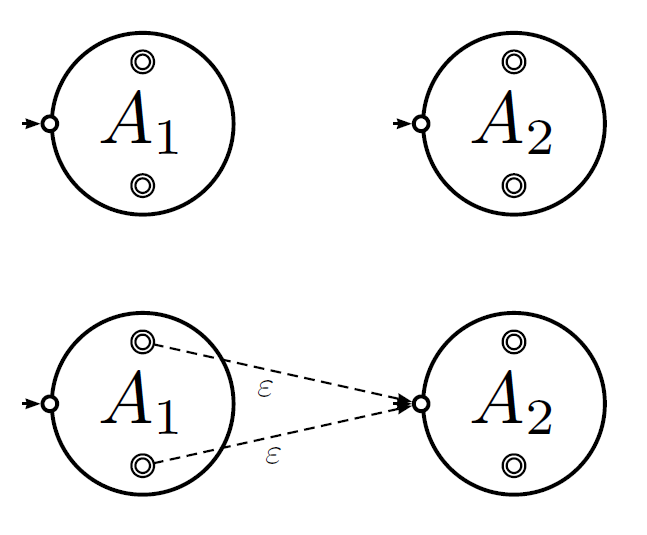
\includegraphics[width=8cm]{img/reg6}
\end{figure}

\begin{figure}[H]
\centering
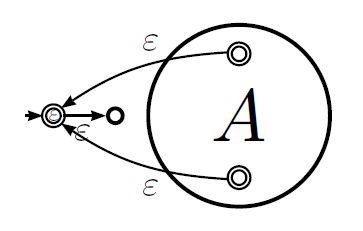
\includegraphics[width=8cm]{img/reg7}
\end{figure}

Sestavíme $\varepsilon$-KNA
$$A= \langle \Sigma,Q_1  \cup Q_2,\delta,\lbrace q_{01} \rbrace,F_2 \rangle$$
s přechodovou funkcí $\delta : (Q_1 \cup Q_2) \times (\Sigma \cup \lbrace \varepsilon \rbrace ) \rightarrow 2^{Q_1 \times Q_2}$
$$
\delta(q,a)=\left\{
\begin{array}{l@{\quad\mbox{}\quad}l}
\lbrace \delta_1(q,a) \rbrace & \text{pokud}\quad q \in Q_1\\
\lbrace \delta_2(q,a) \rbrace & \text{pokud}\quad q \in Q_2\\
\end{array}
\right.
$$
$$
\delta(q,\varepsilon)=\left\{
\begin{array}{l@{\quad\mbox{}\quad}l}
\lbrace q_{02} \rbrace & \text{pokud}\quad q \in F_1\\
\emptyset & \text{pokud}\quad q \notin F_1\\
\end{array}
\right.
$$

\item
\textit{Kleeneho uzávěr}

Pokud je $L$ regulární, pak je $L^*$ regulární.

Předpokládáme, že existuje automat $A$ tak, že $L = L(A)$
\begin{poznamka}
Automat rozpoznávající $L^*$ musí mít možnost dostat se z koncového stavu zpět na začátek.
\end{poznamka}
Pro automat $A = \langle \Sigma, Q, \delta, q_0, F \rangle$ je potřeba zavést nový počáteční stav $q_T \notin Q$. Konstruovaný  $\varepsilon$-KNA bude vypadat následovně:
$$A' = \langle \Sigma, Q \cup \lbrace q_T \rbrace, \delta ', \lbrace q_T \rbrace, F \cup \lbrace q_T \rbrace \rangle$$
s přechodovou funkcí $\delta '$:
$$
\begin{array}{l@{\quad\mbox{}\quad}l}
\delta ' (q,a) = \lbrace \delta (q,a) \rbrace & \text{pokud}\quad q \in Q\\
\delta ' (q,\varepsilon) = \emptyset & \text{pokud}\quad q \in Q \backslash F\\
\delta ' (q,\varepsilon) = \lbrace q_T \rbrace & \text{pokud}\quad q \in F\\
\delta ' (q_T,\varepsilon) = \lbrace q_0 \rbrace & \\
\delta ' (q_T,a) = \emptyset & a \in \Sigma \\

\end{array}
$$
\end{itemize}



\subsection{Další uzávěrové vlastnosti}

\begin{itemize}

\item
\textit{Množinový rozdíl}

Jsou-li $L_1$ a $L_2$ regulární, pak $L_1 \backslash L_2 = L_1 \cap (\Sigma^* \backslash L_2)$ je regulární.

\item
\textit{Kleeneho pozitivní uzávěr}

Je-li $L$ regulární, pak $L^+ = (L^* \backslash \lbrace \varepsilon \rbrace) \cup L$ je regulární.

\item
\textit{N-tá mocnina jazyka}

$L^n$ \ldots plyne z uzavření na produkt

\item
\textit{Jazyk reverzních řetězců}

$L^R = \lbrace w^R \ |\ w \in L \rbrace$



\item
\textit{Jazyk sufixů}

$Sfx(L) = \bigcup_{w \in L} Sfx(w)$


\begin{poznamka}
Všechny stavy jsou označeny za počáteční, aby měl automat možnost skočit do libovolné fáze výpočtu a tím "uhádnout" vynechané znaky řetězce, jehož sufix zkoumáme.
\end{poznamka}

\item
\textit{Jazyk prefixů}
\begin{eqnarray*}
Pfx(L) &=& \bigcup_{w \in L} Pfx(w) \\
Pfx(L) &=& (Sfx(L^R))^R
\end{eqnarray*}
Důkaz plyne z uzavření na Sfx a reverzní řetězec.

\item
\textit{Jazyk infixů}
$$
Ifx(L) = Pfx(Sfx(L))
$$
Důkaz je taktéž zřejmý.
\end{itemize}



%----------------------------------------------------------------------------------------------------------------------
	\subsection{Konečné automaty deterministické a nedeterministické}

\subsubsection{Konečné deterministické automaty}

 KDA realizují analytický (resp. výpočetní) formalismus a představují jakési \uv{jednoduché počítače}.
KDA a jejich činnost jsou charakterizovány několika prvky:
\begin{enumerate}
\item
Vstupem jsou řetězce nad určitou abecedou, která se obvvykle značí $\Sigma$.

\item
Řídící jednotka automatu se skládá z konečně mnoha stavů (aby byla reprezentovatelná v počítačích).

\item
Počátek činnosti automatu představuje okamžik, kdy na vstupu automatu je celý vstupní řetězec a
řídící jednotka je v iniciálním stavu.

\item
Automat vykonává svou primární činnost tím, že přečte ze vstupu aktuální symbol a na základě stavu, ve kterém se právě
nachází se řídící jednotka přepne do jiného stavu a odebere onen přečtený symbol ze vstupního řetězce.

\item
Konec činnosti automatu nastává v případě, že na vstupu již není co číst. Byl tedy zpracován celý
vstupní řetězec. V tomto okamžiku automat nachází v určitém stavu, podle typu stavu následně řekneme, že
automat řetězec přijímá nebo zamítá. Existují tedy přijímací (neboli koncové) stavy a nepřijímací (neboli nekoncové) stavy.
\end{enumerate}

\begin{priklad}
Nyní si ukažme, jak vypadá typický KDA.

\begin{figure}[H]
\begin{center}
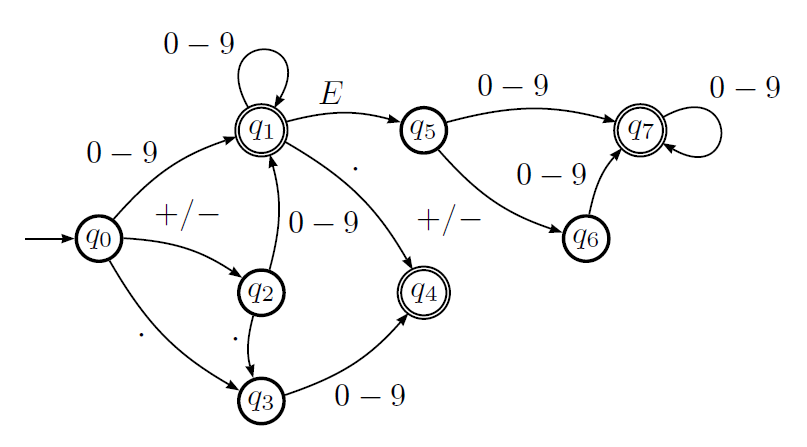
\includegraphics[width=11cm]{img/KDA-priklad}
\end{center}
\end{figure}
\end{priklad}

Dvojitě kroužkovaný stav označuje stav koncový. Šipky mezi jednotlivými stavy označují přechody, přičemž popisek u jednotlivých přechodů
indikuji symbol, který se čte, pokud je tento přechod využit. Automat na obrázku  by přijímal například slovo $13.6E+2$, obecně
jakékoliv číslo kodované v tradiční fixní a pohyblivé notaci s desetinnou tečkou.

\begin{definice}
Konečný deterministický automat s úplnou přechodovou funkcí je struktura:
$$
A = \langle \Sigma, Q, \delta, q_0, F \rangle
$$
Nyní si popišme jednotlivé členy automatu:
\begin{eqnarray*}
\Sigma &=& \text{vstupní abeceda} \\
Q &=& \text{konečná množina stavů} \\
q_0 \in Q &=& \text{počáteční stav} \\
F \subseteq Q &=& \text{množina koncových stavů} \\
\delta &=& \text{zobrazení } \delta:\quad Q \times \Sigma \rightarrow Q \text{, neboli přechodová funkce}
\end{eqnarray*}
U přechodové funkce $\delta$ uvažujeme zápis například $\delta(r, a) = q$, který čteme: \uv{Při vstupním symbolu $a \in \Sigma$ a aktuálním
stavu $r$ přejde automat do nového stavu $q$.}

Předpokládáme, že $Q$ je konečná a $\delta$ je zobrazení.
\end{definice}

\begin{priklad}
Automat s nadefinovanými přechody dle $\delta$ by mohl vypadat například takto:
\begin{eqnarray*}
A &=& \langle \Sigma, Q, \delta, q_0, F \rangle \\
\Sigma &=& \lbrace a, b, c \rbrace \\
Q &=& \lbrace q_0, q_1, q_2, q_3, q_4 \rbrace \\
F &=& \lbrace q_4 \rbrace \\
\delta &=& \lbrace <q_0, a, q_0>, <q_0, b, q_0>, <q_0, c, q_1> \\
& & <q_1, a, q_2>, <q_1, b, q_0>, <q_1, c, q_1> \\
& & <q_2, a, q_0>, <q_2, b, q_3>, <q_2, c, q_1> \\
& & <q_3, a, q_2>, <q_4, b, q_0>, <q_3, c, q_4> \\
& & <q_4, a, q_4>, <q_4, b, q_4>, <q_4, c, q_4> \rbrace
\end{eqnarray*}
\end{priklad}

\subsubsection{Reprezentace KDA}
\textbf{Reprezentace přechodovou tabulkou}\\

\vspace{3mm}

Řádky tabulky představují stavy a sloupce jednotlivé symboly vstupní abecedy. Znak $^*$ označuje, že stav je koncový.
\begin{table}[h]
\begin{center}
\begin{tabular}{r || c | c | c}
 & a & b & c \\
\hline
 $q_0$ & $q_0$ & $q_0$ & $q_1$ \\
 $q_1$ & $q_2$ & $q_0$ & $q_1$ \\
 $q_2$ & $q_0$ & $q_3$ & $q_1$ \\
 $q_3$ & $q_2$ & $q_0$ & $q_4$ \\
 $q_4^*$ & $q_4$ & $q_4$ & $q_4$ \\
\end{tabular}
\end{center}
\caption{Přechodová tabulka pro KDA}
\end{table}


\subsubsection{Reprezentace přechodovým diagramem}

\vspace{3mm}

\begin{figure}[ht]
\begin{center}
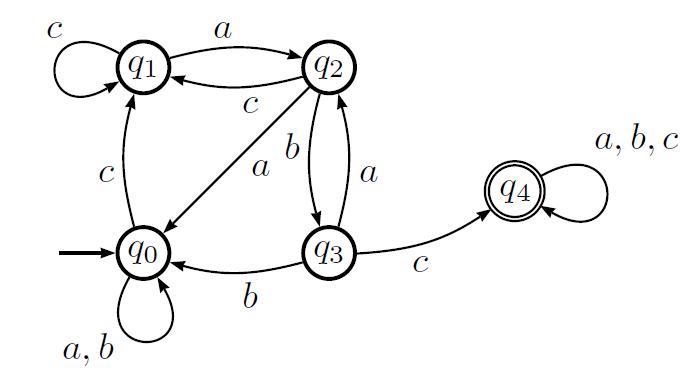
\includegraphics[width=8cm]{img/KDA-priklad2}
\end{center}
\caption{Přechodový diagram pro KDA}
\end{figure}

\subsubsection{Konfigurace a výpočet KDA}

Konfgurace jednoznačně určuje aktuální fázi výpočtu a jsou to dvojice $\langle q, w \rangle, q \in Q, w \in \Sigma^*$, následně
samotná konfigurace $Q \times \Sigma^*$.

Počáteční konfigurace zahrnuje obvykle počáteční stav $q_0$, tedy například $\langle q_0, w \rangle$.

Koncová konfigurace je konfigurací, kdy jsme přečetli celý vstupní řetězec,
tedy $\langle q, \varepsilon \rangle$. Nicméně je třeba rozlišit dva stavy:
\begin{enumerate}
\item
Koncová přijímací konfigurace, pro případ, kdy $q \in F$.

\item
Koncová zamítací konfigurace, pro případ, kdy $q \notin F$.
\end{enumerate}

\begin{definice}
Mějme automat $A = \langle \Sigma, Q, \delta, q_0, F \rangle$ a řetězec $w \in \Sigma^*$. Pak posloupnost
konfigurací $r_i, w_i$ pro $i \in \lbrace 0, 1, \ldots, n \rbrace$ splňující podmínky:
\begin{enumerate}
\item
$r_0$ je počáteční stav automatu $A$.

\item
$w_0 = w$

\item
$w_n = \varepsilon$

\item \label{vypocet-bod-4}
$w_i = a_i w_{i+1}$ a $\delta(r_i, a_i) = r_{i+1}$ pro každé $i \in \lbrace 0,1,\ldots,n-1 \rbrace$
\end{enumerate}
nazveme \textit{výpočet automatu A délky $n$ pro řetězec $w$}.

Popíšme si nyní jeden krok výpočtu, tj. obecně:
$$
\langle r_i, w_i \rangle = \langle r_{i+1}, w_{i+1} \rangle
$$
tj. $w_{i+1}$ vzniknlo z $w_i$ odebráním prvního symbolu, který si označme $a_i$. Do stavu $r_{i+1}$ jsme se dostali ze
stavu $r_i$ při vstupním symbolu $a_i$.
\end{definice}


\begin{priklad}
Typický automatový výpočet vypadá například takto:

\begin{gather*}
\langle q_0 ; accbcabca \rangle \\
\langle q_0 ; ccbcabca \rangle \\
\langle q_1 ; cbcabca \rangle \\
\langle q_1 ; bcabca \rangle \\
\langle q_0 ; cabca \rangle \\
\langle q_1 ; abca \rangle \\
\langle q_2 ; bca \rangle \\
\langle q_3 ; ca \rangle \\
\langle q_4 ; c \rangle \\
\langle q_4 ; \varepsilon \rangle \\
\end{gather*}
\end{priklad}

\begin{veta}
KDA $A$ má pro řetězec délky $n$ jednoznačný výpočet rovněž délky $n$.
\end{veta}

\subsubsection{Rozšířená přechodová funkce pro KDA}

Rozšířená přechodová funkce má rekurzivní předpis:
\begin{gather*}
\delta^*:\quad Q \times \Sigma^* \rightarrow Q \\
\delta^*(q, u) = \lbrace
\begin{array}{l l}
q & \text{pokud } u = \varepsilon \\
\delta^*(\delta(q, a), v) & \text{pokud } u = av, a \in \Sigma, 
\end{array}
\end{gather*}

\begin{veta}\label{veta-kdaaa}
Pro každé $u,v \in \Sigma^* \text{ platí, že } \delta^*(q, uv) = \delta^*(\delta^*(q, u), v)$
\end{veta}


\begin{poznamka}
Automat $A$ přijímá řetězec $w$, pokud $\delta^*(q_0,w) \in F$.
\end{poznamka}

\begin{veta}
Řetězec $w$ je přijat automatem, právě když existuje přijímací výpočet pro $w$.
\end{veta}


Jazyk rozpoznaný konečným deterministickým automatem lze formulovat jako:
$$L(A) = \lbrace w \in \Sigma^* |\quad \delta^*(q_0,w) \in F \rbrace$$

\subsubsection{KDA s neúplnou přechodovou funkcí}

Mějme KDA $A = \langle \Sigma, Q, \delta, q_0, F \rangle$ a upřesněme $\delta$, které se liší.

$\delta$ je neúplná přechodová funkce tvaru $\delta \subseteq Q \times \Sigma \times Q$, přičemž také platí, že
pokud $\langle q, a, r_1 \rangle \in \delta$ a $\langle q,a,r_2 \rangle \in \delta$, pak $r_1 = r_2$ a $\delta:\quad Q \times \Sigma \rightarrow Q$.

Z toho plynou dvě situace:
\begin{enumerate}
\item
$\delta(q, a)$ je definována, $\langle q,a,r \rangle \in \delta$ pro nějaké $r$ takové, že $\delta(q,a) = r$.

\item
$\delta(q,a)$ není definováno, pokud $\langle q, a, r \rangle \notin \delta$ pro žádná $r$.

V grafu se toto projeví tak, že ze stavu $q_i$ nevede žádná hrana pro symbol $a_i$.

Výpočet se liší v bodu \ref{vypocet-bod-4} $w_i = a_i w_{i+1}$ a $\delta(r_i, a_i)$ je definována a $\delta(r_i,a_i) = r_{i+1}$
pro každé $i \in \lbrace 0,1,\ldots,n \rbrace$.
\end{enumerate}

Řetězec $w$ je přijat automatem $A$, právě tehdy, když existuje výpočet $A$ pro $w$, kteý je přijímající.

Následně jazyk rozpoznaný automatem $A$ je $L(A) = \lbrace w \in \Sigma^*| \quad \delta^*(q_0,w) \in F \rbrace$.

\begin{veta}
Ke každému KDA s neúplnou přechodovu funkcí $\delta$ existuje KDA s úplnou přechodovu funkcí $\delta$, který rozpoznává stejný jazyk.
\end{veta}


\subsection{Implementace KDA}
\begin{enumerate}
\item $\delta$ jako dvourozměrné pole - \uv{ďábelsky rychlé}, paměťově náročné
\item $\delta$ jako seznam/hashovací tabulka - vhodné když $|\delta | <<< |Q\times \Sigma |$
\item $\delta$ jako orientovaný graf
\end{enumerate}


\subsubsection{Konečné nedeterministické automaty}

\begin{priklad}
Mějme automat:

\vspace*{40px}
\begin{center}
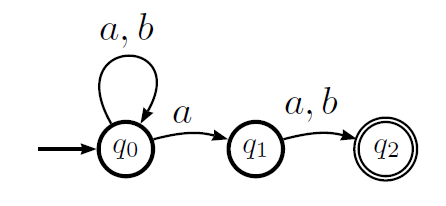
\includegraphics[width=8cm]{img/KDA-priklad3}
\end{center}

Vstupní řetězce: \textit{abba} (nepřijat), \textit{baba} (nepřijat), \textit{baab} (přijat), \textit{bbaa} (přijat).

V případě řetězce \textit{baab} máme dokonce 3 možnosti výpočtu:
\begin{enumerate}
\item
$\langle q_{0}, baab \rangle, \langle q_{0}, aab \rangle, \langle q_{0}, ab \rangle, \langle q_{0}, b \rangle, \langle q_{0}, \varepsilon \rangle \text{ -- končí neúspěchem.}$
\item
$\langle q_{0}, baab \rangle, \langle q_{0}, aab \rangle, \langle q_{1}, ab \rangle, \langle q_{2}, b \rangle \text{ -- končí neúspěchem.}$
\item
$\langle q_{0}, baab \rangle, \langle q_{0}, aab \rangle, \langle q_{0}, ab \rangle, \langle q_{1}, b \rangle, \langle q_{2}, \varepsilon \rangle \text{ -- končí úspěchem.}$ 
\end{enumerate}
Předchozí zápisy můžeme pojmenovat také jako \uv{nedeterministický výpočet.}

Jiným zápisem téhož může být také ten následující.
$$
\langle \lbrace q_{0} \rbrace, baab \rangle, \langle \lbrace q_{0} \rbrace, aab \rangle, \langle \lbrace q_{0}, q_{1} \rbrace, ab \rangle,
\langle \lbrace q_{0}, q_{1}, q_{2} \rbrace, b \rangle, \langle \lbrace q_{0}, q_{2} \rbrace, \varepsilon \rangle
$$ 
\end{priklad}

\begin{definice}
Strukturu $A = \langle \Sigma, Q, \delta, I, F \rangle$ nazvěme \textit{konečným nedeterministickým automatem} nad abecedou $\Sigma$. Pro tuto strukturu následně platí tato tvrzení:
\begin{itemize}
\item
$\Sigma, Q \text{ a } F$ jsou stejné jako u konečného deterministického automatu.
\item
$I\subseteq Q$ označuje množinu počátečních stavů, která by měla být obecně neprázdná.
\item
$\delta$ označuje přechodovou funkci ve tvaru $\delta : Q \times \Sigma \rightarrow 2^{Q}$, tedy $\delta (q, a) = \lbrace r_{1}, \ldots, r_{k} \rbrace$. Totéž slovně: \uv{Automat může při stavu \textit{q} při symbolu \textit{a}
přejít do kteréhokoliv stavu z $\lbrace r_{1}, \ldots, r_{k} \rbrace$.}
\end{itemize}
\end{definice}

\begin{priklad}\label{priklad-3}
\begin{eqnarray*}
\Sigma &=& \lbrace a, b \rbrace \\
P &=& \lbrace q_{0}, q_{1}, q_{2}, q_{3} \rbrace \\
I &=& \lbrace q_{0}, q_{3} \rbrace \\
F &=& \lbrace q_{2} \rbrace 
\end{eqnarray*}
Následně přechodová funkce:
\begin{eqnarray*}
\delta =&
\lbrace
\langle q_{0}, a, \lbrace q_{0},q_{1} \rbrace \rangle,
\langle q_{0}, b, \lbrace q_{0} \rbrace \rangle,
\langle q_{1}, a, \lbrace q_{2} \rbrace \rangle,
\langle q_{1}, b, \lbrace q_{2} \rbrace \rangle, \\
& \langle q_{2}, a, \emptyset \rangle,
\langle q_{2}, b, \emptyset \rangle,
\langle q_{3}, a, \emptyset \rangle,
\langle q_{3}, b, \lbrace q_{1} \rbrace \rangle 
\rbrace
\end{eqnarray*}
\end{priklad}

\subsubsection{Reprezentace KNA}
Předchozí příklad číslo \ref{priklad-3} lze reprezentovat několika způsoby:
\begin{enumerate}
\item
\textit{Přechodová tabulka}, která ve svém těle obsahuje množiny stavů.
\begin{table}[h]
\begin{center}
\begin{tabular}{ r || c | c }                   
   & a & b \\
   \hline
   $ \rightarrow q_{0} $ & $ \lbrace q_{0},q_{1} \rbrace $ & $ \lbrace q_{0} \rbrace $ \\
   $ q_{1} $ & $ \lbrace q_{2} \rbrace $ & $ \lbrace q_{2} \rbrace $ \\
   $ q_{2} * $ & $ \emptyset $ & $ \emptyset $ \\
   $ \rightarrow q_{3} $ & $ \emptyset $ & $ \lbrace q_{1} \rbrace $ \\ 
\end{tabular}
\end{center}
\caption{Přechodová tabulka s množinami stavů}
\end{table}

\item
\textit{Diagram}, který automat demonstruje v grafičtější podobě.

\begin{center}
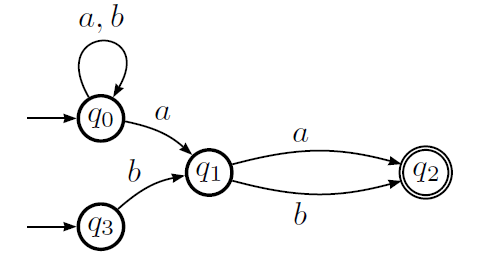
\includegraphics[width=8cm]{img/KNA}
\end{center}


\end{enumerate}


\subsubsection{Nedeterministický výpočet}
Nyní si popišme \textit{nedeterministický výpočet}, který je definován následujícími věcmi:
\begin{itemize}
\item
Konfigurace, což je dvojice ve tvaru $\langle \textit{stav}, \textit{řetězec} \rangle $.
\item
Počáteční konfigurace ve tvaru $\langle q, w \rangle \text{ kde } q \in I$.
\item
Koncová konfigurace ve tvaru $\langle q, \varepsilon \rangle $.
\item
Koncová přijímací konfigurace $\langle q, \varepsilon \rangle \text{ kde } q \in F$.
\end{itemize}

\begin{definice}
Mějme $A = \langle \Sigma, Q, \delta, I, F \rangle  \text{ a } w \in \Sigma^{*}$. Pak posloupnost konfigurací $\langle r_{i}, w_{i} \rangle \text{ pro } i = \lbrace 0, \ldots, n \rbrace $ splňující podmínky:
\begin{gather}
r_{0} \in I \\
w_{0} = w \\
w_{n} = \varepsilon \\
w_{i} = a_{i}w_{i+1} \text{ a } r_{i+1} \in \delta (r_{i}, a_{i}) \text{ pro } i = \lbrace 0, \ldots,  n-1 \rbrace
\end{gather}
nazveme \textit{nedeterministický výpočet}.
\end{definice}


\subsubsection{Rozšířená přechodová funkce}
\begin{definice}
Rozšířená přechodová funkce má tvar:
\begin{gather*}
\delta^{*} : 2^{Q} \times \Sigma^{*} \rightarrow 2^{Q} \\
\delta^{*}(R, w) = \left\lbrace
\begin{array}{l l}
R & \text{ pokud } w = \varepsilon \\
\delta^{*}(\bigcup\limits_{q \in R} \delta(q, a), u) & \text{ pokud } w = au\text{, kde } a \in \Sigma, u \in \Sigma^{*} \\
\end{array}
\right\rbrace
\end{gather*}
\end{definice}

\begin{veta}
Platí $\delta^{*}(R,w) = \delta^{*}(\delta^{*}(R,u),v), \forall R \subseteq Q, uv \in \Sigma^{*}$.
\end{veta}


\begin{veta}
Platí následující tvrzení:
$$
\delta^{*}(\bigcup\limits_{i=1}^{k} R_{i},w) = \bigcup\limits_{i=1}^{k} \delta^{*}(R_{i},w) \text{ pro každé} R_{i} \subseteq Q, w \in \Sigma^{*}
$$
\end{veta}


\subsubsection{Řetězce přijímané KNA}
KNA $A$ přijímá řetězec $w$, pokud $\delta^{*}(I,w) \cap F \neq \emptyset$.
Navíc jazyk, přijímaný KNA $A$ si definujme jako $L(A) = \lbrace w \in \Sigma^{*} | \delta^{*}(I,w) \cap F \neq \emptyset \rbrace$.

\begin{veta}
Platí, že $w \in L(a)$ právě tehdy, když KNA $A$ má přijímací výpočet pro $w$.
\end{veta}


	\subsection{Regulární výrazy}

\begin{definice}
Nechť je dána $\Sigma = \lbrace a_{1}, \ldots, a_{k} \rbrace$. Pak regulární výraz na $\Sigma$ je:
\begin{enumerate}
\item
$\emptyset$

\item
$\varepsilon$

\item
symboly $a_{1}, \ldots, a_{k}$

\item
pokud $R_{1}, R_{2}$ jsou RV, pak $(R_{1}|R_{2})$ je RV

\item
pokud $R_{1}, R_{2}$ jsou RV, pak $(R_{1}R_{2})$ je RV

\item
pokud $R$ je RV, pak $R^{*}$ je RV
\end{enumerate}
\end{definice}

\begin{priklad}
Podívejme se na následující výrazy a rozhodněme, zda-li jsou regulární:

\begin{itemize}
\item
$((ab)c)^{*}$, $((a|b)c)^{*}$ -- jsou RV

\item
$a^{*}b)$, $a||b$ -- nejsou RV
\end{itemize}
\end{priklad}
\begin{poznamka}
Priorita $| , \circ , *$ je stejná jako (po řadě) $+ , \cdot , ^{-1}$ v aritmetických výrazech.
\end{poznamka}
\subsubsection{Jazyky generované regulárními výrazy}

\begin{definice}
Nechť \textit{R} je RV nad $\Sigma$. Pak $L(R) \subseteq \Sigma^{*}$. Pak také platí:

\begin{enumerate}
\item\label{jazyky-1}
$L(R) = \emptyset$, pokud $R = \emptyset$.

\item
$L(R) = \lbrace \varepsilon \rbrace$, pokud $R = \varepsilon$.

\item\label{jazyky-3}
$L(R) = \lbrace a_{i} | \quad \text{pokud } R=a_{i} \rbrace$.

\item\label{jazyky-4}
$L(R) = L(R_{1}) \cup L(R_{2})$, pokud $R=\lbrace R_{1} | R_{2} \rbrace$. 

\item\label{jazyky-5}
$L(R) = L(R_{1}) \circ L(R_{2})$, pokud $R=\lbrace R_{1}\circ R_{2} \rbrace$.

\item\label{jazyky-6}
$L(R) = L(R_{1})^{*} $, pokud $R = R_{1}^{*}$.
\end{enumerate}
\end{definice}

\begin{veta}
Každý regulární výraz lze převést na konečný automat.
\end{veta}

\begin{veta}
Každý jazyk generovaný regulárním výrazem je regulární.
\end{veta}



\begin{veta}
Každý regulární jazyk lze generovat regulárním výrazem.
\end{veta}
%%%%%%%%%%%%%%%%%%%%%%%%%%%%%%%%%%%%%%%%%
	\subsection{Automaty s epsilon-přechody}
Značíme $\varepsilon$-KNA.
\begin{priklad}\label{priklad-5}
Zde je jeden motivační příklad na úvod.

\begin{figure}[H]
			\centering
			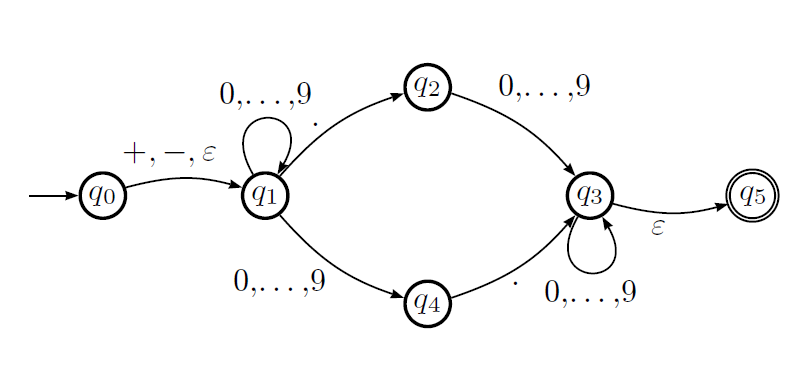
\includegraphics[width=8cm]{img/e}
			\end{figure}

\end{priklad}

\begin{definice}
Nedeterministický konečný automat s $\varepsilon$-přechody je struktura $ \langle \Sigma,Q,\delta,I,F \rangle $,
kde $\Sigma,Q,\delta,I,F$ mají stejný význam jako u KNA. $\delta$ je přechodová funkce $\delta : Q \times (\Sigma \cup \lbrace \varepsilon \rbrace ) \rightarrow 2^Q$.
\end{definice}

Fakt $\delta (q,a) = \lbrace r_1,\ldots,r_k \rbrace $ čteme: \uv{automat \textit{A} při čtení symbolu \textit{a} přejde ze stavu \textit{q} do některého ze stavů $r_1,\ldots,r_k$.}

Fakt $\delta (q,\varepsilon) = \lbrace r_1,\ldots,r_k \rbrace $ čteme: \uv{automat \textit{A} přejde samovolně ze stavu \textit{q} do některého ze stavů $r_1,\ldots,r_k$.}

\subsection{Reprezentace $\varepsilon$-KNA}

\begin{enumerate}

\item
\textit{Přechodová tabulka}, vypadá stejně jako u KNA s tím, že přidáme jeden sloupec, ve kterém budeme zaznamenávat $\varepsilon$-přechody.

Takto bude vypadat předchozí př\'iklad číslo \ref{priklad-5}, reprezentovaný pomocí tabulky.

\begin{table}[h]
\begin{center}
\begin{tabular}{ r || c | c | c | c }                   
   & +,- & . & $0,\ldots,9$ & $\varepsilon$ \\
   \hline
   $ \rightarrow q_{0} $ & $ \lbrace q_{1} \rbrace $ & $ \emptyset $ & $ \emptyset $ & $ \lbrace q_{1} \rbrace $\\
   $ q_{1} $ & $ \lbrace q_{2} \rbrace $ & $ \emptyset $ & $ \lbrace q_{1},q_{2} \rbrace $ & $\emptyset$ \\
   $ q_{2} $ & $ \emptyset $ & $ \emptyset $ & $\lbrace q_{3} \rbrace$ & $ \emptyset $ \\
   $ q_{3} $ & $ \emptyset $ & $ \emptyset $ & $\lbrace q_{3} \rbrace$ & $\lbrace q_{5} \rbrace$ \\
   $ q_{4} $ & $ \emptyset $ & $\lbrace q_{3} \rbrace$ & $\emptyset$ & $ \emptyset $ \\
   $ q_{5}^* $ & $ \emptyset $ &  $ \emptyset $ & $\emptyset$ & $ \emptyset $ 
\end{tabular}
\end{center}
\caption{Přechodov\'a tabulka pro \ref{priklad-5}. přiklad}
\end{table}

\item
\textit{Přechodový diagram}, u kterého mohou být některé hrany ohodnoceny $\varepsilon$. Viz příklad \ref{priklad-5}.

\end{enumerate}

\subsubsection{Nedeterministický výpočet}
Pojem \textit{konfigurace} pro nás zůstává stejný, jedná se stále o dvojici $\langle \textit{stav,řetězec} \rangle$.

\begin{definice}
Mějme automat $A = \langle \Sigma,Q,\delta,I,F \rangle$ a řetězec $w \in \Sigma^*$. Posloupnost konfigurací $\langle r_i,w_i \rangle$ pro $i=0,\ldots,n$ splňující podmínky:
\begin{enumerate}
\item
$r_{0} \in I, w_0=w$
\item
$w_{n} = \varepsilon$
\item
pro každé $i=0,\ldots,n$
\begin{enumerate}
\item
$w_i = aw_{i+1}, r_{i+1} \in \delta(r_i,a)$
\item
$w_i=w_{i+1} , r_{i+i} \in \delta(r_i,\varepsilon)$
\end{enumerate}
\end{enumerate}

\end{definice}

\subsubsection{$\varepsilon$-uzávěry množin stavů}

Je dána množina stavů $R \subseteq Q$, jež se nazývá $\varepsilon$-uzavřená,
pokud $ \delta (q,\varepsilon) \subseteq R$ pro každý stav $ q \in R$.

\begin{priklad}
Lze ukázat na našem příkladě \ref{priklad-5}.

$\lbrace q_0 \rbrace $ není $\varepsilon$-uzavřená protože $\delta(q_0,\varepsilon) = \lbrace q_1 \rbrace \nsubseteq \lbrace q_0 \rbrace$

$\lbrace q_0,q_1 \rbrace$ je $\varepsilon$-uzavřená
\end{priklad}

\subsubsection{Tvorba $\varepsilon$-uzávěru}

\begin{enumerate}
\item
Mějme $\varepsilon$-uzávěr $R$.

\item
Prohlašme, že $E_0=R$ a následně pro $i \geq 1$ tvrďme, že:

\begin{itemize}
\item
$E_i=E_{i-1} \cup \lbrace \delta (q,\varepsilon) | q \in E_{i-1}\rbrace$

\item
$E_A(R)=\bigcup_{i=0}^\infty E_i$

\item
$E_0 \subseteq E_1 \subseteq E_2 \subseteq \ldots \subseteq E_A(R)$
\end{itemize}
\end{enumerate}

\begin{poznamka}
Vzhledem ke konečnosti množiny $E_A(R)$ musí existovat index $k$, pro který platí $E_k = E_{k+1} = \ldots = E_A(R)$
\end{poznamka}

Můžeme pozorovat, že $E_A(R)$ není jen $\varepsilon$-uzavřená, ale je také \textit{nejmenší} $\varepsilon$-uzavřená. Z toho můžeme vyvodit, že 

$$E_A:2^Q \rightarrow 2^Q$$

je \textit{uzávěrový} operátor.

\subsubsection{Rozšířená přechodová funkce}

Pro automat $A = \langle \Sigma,Q,\delta,I,F \rangle$ je rozšířená přechodová funkce definovaná jako

$\delta^*:2^Q \times \Sigma^* \rightarrow 2^Q$

$$
\delta^*(R,w)=\left\{
\begin{array}{l@{\quad\mbox{}\quad}l}
E_A(R) & \text{pokud}\quad w=\varepsilon\\
\delta^*(E_A(\bigcup_{q \in E_A(R)}\delta(q,a),u))& \text{pokud}\quad w=au,a\in\Sigma,u\in\Sigma^*\\
\end{array}
\right.
$$

\begin{veta}
Pro libovolné množiny $R_i \subseteq Q \quad (i=1,\ldots,k)$ platí:

$\bigcup_{i=1}^k E_A(R_i)=E_A(\bigcup_{i=1}^kR_i)$
\end{veta}



\subsubsection{Přijímaný řetězec $\varepsilon$-KNA}

Nechť $A=\langle\Sigma,Q,\delta,I,F\rangle$ je $\varepsilon$-KNA. Řetězec $w \in \Sigma^*$ nazýváme řetězec \textit{přijímaný} $A$, pokud

$\delta^*(I,w) \cap F \neq \emptyset$

jinak $w$ nazýváme řetězec \textit{zamítaný} $A$.

Jazyk přijímaný A: $L(A) = \lbrace w \in \Sigma^{*} | \delta^{*}(I, w) \cap F \neq \emptyset \rbrace$ 
\paragraph{Ekvivalence s KDA}

\begin{veta}
Ke každému $\varepsilon$-KNA  $A=\langle\Sigma,Q,\delta,I,F\rangle$ existuje KNA $A^S=\langle\Sigma,Q,\delta^S,I^S,F\rangle$ takový, že $L(A)=L(A^S)$.
\end{veta}
 



%%%%%%%%%%%%%%%%%%%%%%%%%%%%%%%%%%%%%%%
	\subsection{Minimalizace konečného deterministického automatu}


\begin{poznamka}
Pro regulární jazyk $L$ existuje více, než jeden automat $A$ tak, že $L = L(A)$ a navíc můžeme mít $A_{1}, A_{2}$ tak, že
$L(A_{1}) = L(A_{2})$, ale $|Q_{1}| < |Q_{2}|$.
\end{poznamka}

\subsubsection{Zprava invariantní ekvivalence}

\begin{definice}
Předpokládejme, že máme $A = \langle \Sigma, Q, \delta, q_{0}, F \rangle$ a relaci ekvivalence $\Theta \subseteq Q \times Q$ nazveme
\textit{zprava invariantní ekvivalencí} vzhledem k $\delta$, pokud platí, že $\langle q,r  \rangle \in \Theta \text{ a } a \in \Sigma$,
pak $\langle  \delta(q, a), \delta(r, a) \rangle \in \Theta$.
\end{definice}

Pravá invariance reprezentuje přirozenou vlastnost, kterou musí mít relace nerozlišitelnosti stavů.

Mezními případy invariantních relací zprava jsou:
\begin{enumerate}
\item 
identita $\Theta = \lbrace \langle q,q \rangle | \quad q \in Q \rbrace$
\item
$\Theta = Q \times Q$
\end{enumerate}

\subsubsection{Faktorizace automatu}

\begin{definice}
Mějme KDA $A = \langle \Sigma, Q, \delta, q_{0}, F \rangle$ a zprava invariantní ekvivalenci $\Theta$ vzhledem k
$\delta$, pak zavedeme $A/\theta = \langle \Sigma, Q/\Theta, \delta^{A/\Theta}, [q_{0}]_{\Theta}, F^{A/\Theta} \rangle$, kde
$$\delta^{A/\Theta} = ([q]_{\Theta}, a) = [\delta(q, a)]_{\Theta} \text{ a } F^{A/\Theta} = \lbrace [q]_{\Theta} | \quad q \in F \rbrace$$
\end{definice}

\begin{veta}\label{veta-aut}
Automat $A$ je dobře definovaný KDA.
\end{veta}



Obecně $L(A/\Theta) \neq L(A)$. Snažíme se najít co největší $\Theta$, tak aby tato rovnost platila.

\begin{priklad}
$\Theta = Q \times Q$

\begin{figure}[H]
			\centering
			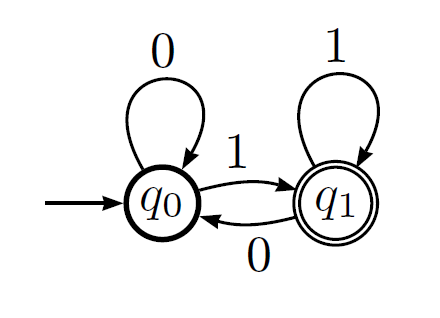
\includegraphics[width=5cm]{img/min1}
			\end{figure}

\end{priklad}

\begin{veta}\label{veta-x2}
Platí, že $(\delta^{A/\Theta})^*([q]_\Theta,x)=[\delta^*(q,x)]_\Theta$ pro každý $x \in \Sigma^*$.
\end{veta}

\begin{definice}
Mějme KDA $A = \langle \Sigma, Q, \delta, q_{0}, F \rangle$ s úplnou přechodovou funkcí.
Pro stavy $q, r \in Q$ položme $q \equiv_{A} r$, pokud pro každ\'y řetězec $x \in \Sigma{*}$ plat\'i, že $\delta^{*}(q,x) \in F$,
právě když $\delta^{*}(r,x) \in F$.
\end{definice}

\begin{veta}\label{veta-zprava}
$\equiv_{A}$ je zprava invariantní operace.
\end{veta}

\begin{veta}\label{veta-4}
Pro $A/ \equiv_{A}$ a stav $q \in Q$ plat\'i, že $q \in F$ pr\'avě, když $[q]_{\equiv_{A}} \in F^{A/ \equiv_{A}}$.
\end{veta}

\begin{dusledek}
KDA $A$ nazveme redukovan\'y, pokud je $\equiv_{A}$ identita.
\end{dusledek}

\begin{veta}
KDA $A/ \equiv_{A}$ je redukovaný.
\end{veta}

\begin{veta}
$L(A) = L(A/ \equiv_{A})$, což plyne užit\'im vět \ref{veta-4} a \ref{veta-x2}.
\end{veta}

\begin{dusledek}
Obecně plat\'i, že $L(A) \subseteq L(A/ \Theta)$.
\end{dusledek}

\begin{veta}
Pokud je každ\'y stav automatu $A$ dosažiteln\'y, pak m\'a $A/ \equiv_{A}$ tak\'e každ\'y stav dosažiteln\'y.
\end{veta}

\subsubsection{Algoritmus pro hled\'an\'i redukovan\'eho automatu}

\begin{enumerate}
\item
Označ\'ime $A/ \equiv_{A} \text{jako } A^{R}$, konstruujeme posloupnost rozkladů na $Q$ tak, že $\varphi_{1}, \varphi_{2}, \ldots, \varphi_{i} = \varphi_{i+1}$,
kde $\varphi_{1} = \lbrace F, Q \setminus F \rbrace$

\item
Při odvozen\'i rozkladů $\varphi_{i}$ z $\varphi_{i-1}$ postupujeme n\'asledovně:

Pro $\forall R \in \varphi_{i-1}$ provedeme:
\begin{enumerate}
\item
Vezmeme libovoln\'y stav $r \in R$.

\item
Polož\'ime $S = \lbrace s \in R | \text{ pro každ\'e } a \in \Sigma \text{ plat\'i tak\'e, že }\delta(S, a) \in [\delta(R, a)] \rbrace$.

\item
Pokud $S = R$, pak vlož\'ime $R$ do $\varphi_{i}$, pokud $S \subseteq R$, pak vlož\'ime $S$ a $R \setminus S$ do $\varphi_{i}$.
\end{enumerate}
\end{enumerate}

\begin{veta}
Korektnost algoritmu pro nalezen\'i $\equiv_{A}$: pokud $\varphi_{i} = \varphi_{i+1}$, pak $\varphi_{i} = Q/ \equiv_{A}$.
\end{veta}


\begin{priklad}
Mějme v\'yraz $b(ab)^{*}ba^{*}$. D\'ale
\begin{eqnarray*}
\varphi_{1} &=& \lbrace \lbrace q_{0},q_{1},q_{2},q_{3},q_{5} \rbrace, \lbrace q_{4}, q_{6} \rbrace \rbrace \\
\varphi_{2} &=& \lbrace \lbrace q_{0},q_{1},q_{3} \rbrace, \lbrace q_{2}.q_{5} \rbrace, \lbrace q_{4}, q_{6} \rbrace \rbrace \\
\varphi_{3} &=& \lbrace \lbrace q_{0},q_{3} \rbrace, \lbrace q_{1} \rbrace, \lbrace q_{2}.q_{5} \rbrace, \lbrace q_{4}, q_{6} \rbrace \rbrace \\
\end{eqnarray*}
\begin{figure}[H]
			\centering
			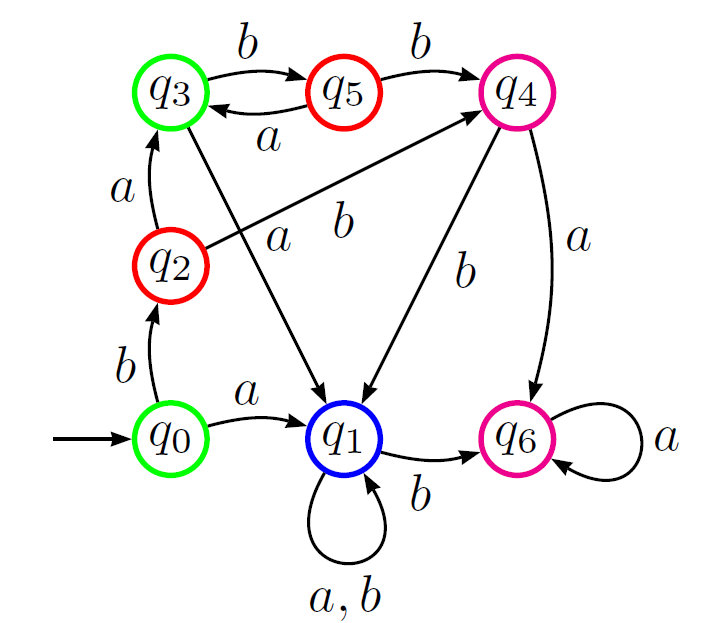
\includegraphics[width=8cm]{img/min2}
			\caption{$q_4$ a $q_6$ jsou přijímací (šipka mezi $ q_1$ a $q_6$  má být obráceně)}
			\end{figure}

N\'asledně rozklady:
\begin{figure}[H]
			\centering
			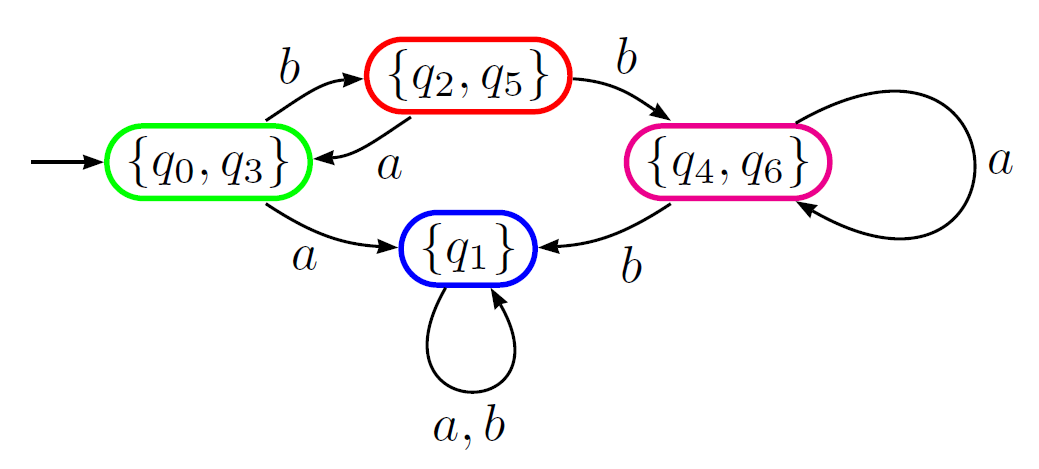
\includegraphics[width=8cm]{img/min3}
			\end{figure}

\vspace*{30px}
\begin{table}[h]
\begin{center}
\begin{tabular}{c||c|c|c|c|c|c|c}
& $q_0$ & $q_1$ & $q_2$ & $q_3$ & $q_4$ & $q_5$ & $q_6$ \\
\hline
$q_0$ & * & X & X & * & X & X & X \\
\hline
$q_1$ & - & * & X & X & X & X & X \\
\hline
$q_2$ & - & - & * & X & X & * & X \\
\hline
$q_3$ & - & - & - & * & X & X & X \\
\hline
$q_4$ & - & - & - & - & * & X & * \\
\hline
$q_5$ & - & - & - & - & - & * & X \\
\hline
$q_6$ & - & - & - & - & - & - & * \\
\end{tabular}
\end{center}
\caption{Tabulkový popis rozkladů stavů}\label{tabulka-x}
\end{table}
%\end{center}
V tabulce \ref{tabulka-x} se objevují znaky \textit{X} na pozicích, pro které platí, že:
\begin{eqnarray*}
T[q,x] &\text{ kde platí }& q \in F, x \notin F \\
&\text{ nebo }& q \notin F, x \in F
\end{eqnarray*}
Projdeme pr\'azdn\'a m\'ista, $T[q,r] = \text{\uv{pr\'azdno, pokud} } \exists a \in \Sigma \text{ tak, že:}$
\begin{itemize}
\item
buď $T[\delta(q,a),\delta(r,a)] = X$
\item
nebo $T[\delta(r,a),\delta(q,a)] = X$
\end{itemize}
Pokud ano, tak \uv{X} na pozici $[q,r]$.
\end{priklad}

\subsubsection{Izomorfismus automatů}
Pro KDA $A_1$ a $A_2$ mějme zobrazen\'i
$$
h: \quad Q_1 \rightarrow Q_2
$$
a toto zobrazení označme jako \textit{izomorfismus}, pokud platí:
\begin{enumerate}
\item
Zobrazení $h$ je bijektivní.
\item
Počáteční stav automatu $A_1$ e zobrazí na počáteční stav automatu $A_2$.
\item
Pro všechna $q \in Q$ platí, že $Q \in F_1$ právě, pokud $q \in F_2$.
\item
Zobrazení $h$ je kompatibilní s přechodovou funkcí.
\end{enumerate}


\begin{veta}
Jsou-li dva automaty izomorfní, pak $L(A_1) = L(A_2)$.
\end{veta}

\begin{definice}
Mějme regulární jazyk L, pak KDA s úplnou přechodovou funkcí je \textit{minimálním automatem} pro $L$,
pokud $L(A) = L$ a pro každý KDA $B$ takový, že $L(B) = L$ platí, že $B$ má tolik stavů jako $A$.
\end{definice}

\begin{veta}
Je-li automat $A$ minimální pro jazyk $L$, pak je \textit{redukovaný}a nemá nedosažitelné stavy.
\end{veta}

\begin{veta}
Pokud jsou automaty $A, B$ KDA bez nedosažitelných stavů a pokud jsou tyto automaty navíc redukované a
existuje stejný jazyk, který generují, pak jsou izomorfní.
\end{veta}

\begin{veta}
$A$ je minimální automat pro jazyk $L$ právě tehdy, když $A$ neobsahuje nedosažitelné stavy a je redukovaný.
\end{veta}



%%%%%%%%%%%%%%%%%%%%%%%%%%%%%%%%%%%%%%%
	\subsection{Pumping lemma}



\begin{poznamka}
Jen drobné upozornění na začátek: jedná se o tvrzení ve tvaru když $\rightarrow$ pak, tj. "Pokud je $L$ regulární, pak $\ldots$"
\end{poznamka}

\begin{veta}
Nechť $L$ je regulární jazyk nad $\Sigma$. Pak existuje $n \in \mathbb{N}$ tak, že pro každý řetězec $w \in L$ délky alespoň $n$ platí, že existují $x,y,z \in \Sigma^*$ tak, že jsou splněny podmínky:
\begin{enumerate}
\item
$w = xyz$
\item
$|xy| \le n$
\item
$y \neq \varepsilon$
\item
pro každé $i \ge 0$ platí, že $xy^iz \in L$
\end{enumerate}
\end{veta}


\begin{priklad}\label{priklad-reg}
 Jazyk $L = \lbrace a^{n}b^{n} | \quad \text{ kde } n \in N \rbrace$ není regulární.
\end{priklad}


	\subsection{Bezkontextové jazyky a jejich vlastnosti (uzávěrové vlastnosti, jednoznačnost)}

V této části se vrátíme k problematice bezkontextových gramatik. Před dalším čtením je potřeba ovládat základní pojmy, zejména
\begin{itemize}

\item
Bezkontextové gramatiky
\item
Bezkontextové jazyky
\item
P-derivace
\item
Odvozování řetězců
\item
Věty a větné formy

\end{itemize}

Navíc si zavedeme duální pojem k derivaci - \textit{redukci}.
\begin{definice}
Řetězec $v$ lze redukovat na řetězec $u$, pokud $u \Rightarrow_G^* v$. Značíme
$v \Leftarrow_G^* u$. 
\end{definice}
V následujícím příkladě si ukážeme problém nejednoznačnosti bezkontextových gramatik.
\begin{priklad}\label{priklad-6}
Mějme gramatiku:

$\begin{array}{l}
G=\langle N,\Sigma,P,S \rangle \\
\Sigma = \lbrace a,b,c,0,1,+,-,*,/,(,) \rbrace \\
N = \lbrace S,E,C,V \rbrace \\
\end{array}\\
\begin{array}{l l}
P= \lbrace &S \rightarrow E, \\
& E \rightarrow E*E|E/E|E+E|E-E|-E|C|V|(E), \\
& C \rightarrow 0C|1C|0|1, \\
& V \rightarrow aV|bV|cV|a|b|c \quad \rbrace
\end{array}
$

Uvažujme větu $w=ac*1-c$. K ní se lze dostat buď:

$
S \Rightarrow_G E \Rightarrow_G E*E \Rightarrow_G V*E \Rightarrow_G V*E-E \Rightarrow_G V*E-V \Rightarrow_G aV*E-V \Rightarrow_G ac*E-V \Rightarrow_G ac*C-V \Rightarrow_G ac*C-c \Rightarrow_G \textit{ac*1-c}
$

nebo

$
S \Rightarrow_G E \Rightarrow_G E*E \Rightarrow_G V*E \Rightarrow_G aV*E \Rightarrow_G ac*E \Rightarrow_G ac*E-E \Rightarrow_G ac*C-E \Rightarrow_G ac*1-E \Rightarrow_G ac*1-V \Rightarrow_G \textit{ac*1-c}
$

Ačkoliv odvozujeme stejnou větu, můžeme zde pozorovat jakousi nejednoznačnost, způsobenou tím, že neterminály derivujeme v libovolném pořadí.
\end{priklad}
Tento problém bychom mohli vyřešit použitím tzv. lineární bezkontextové gramatiky, tedy takové, jejíž odvozovací pravidla obsahují pouze jeden neterminální symbol na pravé straně.
\begin{priklad}Lineární gramatika může vypadat např. takto: \\
$\begin{array}{l}
G=\langle N,\Sigma,P,S \rangle \\
\end{array}\\
\begin{array}{l l}
P= \lbrace &S \rightarrow abB, \\
& A \rightarrow aaBb|\varepsilon, \\
& B \rightarrow bbAa \quad \rbrace
\end{array}
$

$\ L(G) = \lbrace ab(bbaa)^nbba(ba)^n\ |\ n \ge0 \rbrace$
\end{priklad}

Ovšem k nejednoznačnosti může stejně dojít, pokud by se z různých neterminálních symbolů daly odvodit stejná slova.

\begin{priklad}
Příklad nejednoznačné lineární gramatiky: \\
$\begin{array}{l}
G=\langle N,\Sigma,P,S \rangle \\
\end{array}\\
\begin{array}{l l}
P= \lbrace &S \rightarrow aA\ |\ aB, \\
& A \rightarrow bA|a, \\
& B \rightarrow bB|a \quad \rbrace
\end{array}
$

Uvažujme slovo $w=abba$, ke kterému lze dojít buď:

$S \Rightarrow_G aA \Rightarrow_G abA \Rightarrow_G abbA \Rightarrow_G abba$

nebo:

$S \Rightarrow_G aB \Rightarrow_G abB \Rightarrow_G abbB \Rightarrow_G abba$
\end{priklad}

Mějme bezkontextovou gramatiku $G = \langle N,\Sigma,P,S \rangle$.

\begin{definice}
P-derivace $x_0,\ldots,x_k$ se nazývá \textit{nejlevější} P-derivace, pokud pro každé $i \in \lbrace 1,\ldots,k \rbrace$ platí, že $x_{i-1}$ je ve tvaru $uAv$, kde $u \in \Sigma^*,A\in N,v \in (\Sigma \cup N)^*$ a $x_i$ je ve tvaru $uyv$, kde $A \rightarrow y \in P$.
\end{definice}

\begin{poznamka}
Řetězci $u$ se říká uzavřená forma a řetězci $Av$ otevřená forma (větné formy $uAv$).\\
Odvození pomocí nejlevější derivace značíme $u \Rightarrow_{G,l} v$.
\end{poznamka}

\begin{veta}
Mějme $v \in \Sigma^*$ a $X \in N$. Pokud existuje P-derivace $X,\ldots,v$, pak existuje nejlevější P-derivace $X,\ldots,v$ používající stejnou množinu pravidel jako výchozí P-derivace.
\end{veta}

\begin{priklad}
Uvažujme gramatiku z příkladu \ref{priklad-6}

$S \Rightarrow_G^* E+C$ tady problém není\\
$S \Rightarrow_{G,l}^* E+C$ tento výraz už smysl nedává. Pomocí nejlevější derivace bychom zákonitě museli nejdříve derivovat $E$ na levé straně výrazu $E+E$
\end{priklad}

\begin{poznamka}
Lze zavést duálně nejpravější derivaci.
\end{poznamka}

\begin{priklad}
Zase se odkážeme na příklad \ref{priklad-6}.

Výraz $10+(ca*110)$ má jedinou nejlevější derivaci

Naopak $a+10*c$ jich má několik:

$S \Rightarrow_{G,l} E \Rightarrow_{G,l} E+E \Rightarrow_{G,l} V+E \Rightarrow_{G,l} a+E \Rightarrow_{G,l} a+E*E \Rightarrow_{G,l} a+C*E \Rightarrow_{G,l} a+1C*E \Rightarrow_{G,l} a+10*E \Rightarrow_{G,l} a+10*V \Rightarrow_{G,l} a+10*c$

nebo:

$S \Rightarrow_{G,l} E \Rightarrow_{G,l} E*E \Rightarrow_{G,l} \ldots \Rightarrow_{G,l} a+10*c$ (už ve druhém odvození můžeme pozorovat rozdíl)

Je to způsobeno jinou nejednoznačností než tou, kterou jsme eliminovali pomocí nejlevější derivace.
\end{priklad}

\subsubsection{Derivační stromy}

Slouží ke grafickému znázornění nejlevějších derivací. Mějme gramatiku $G = \langle N,\Sigma,P,S \rangle$.

\begin{definice}
Derivačním stromem slova $x \in (\Sigma \cup N)^*$ z $X \in N$ podle pravidel z $G$ je každý strom splňující:
\begin{enumerate}
\item 
každý vnitřní uzel je ohodnocen neterminálem
\item
kořen je ohodnocen $X$
\item
pokud je vnitřní uzel označený $A\in N $ a jeho potomci jsou zleva doprava označeni $X_1,\ldots,X_k \in N\cup \Sigma$ pak existuje pravidlo $A \rightarrow X_1 \cdots X_k \in P$
\item
zřetězením hodnot v listech při průchodu stromu do hloubky a zleva doprava získáme řetězec $x$
\end{enumerate}
\end{definice}

\begin{priklad}
Opět pracujeme s gramatikou z příkladu \ref{priklad-6}.

$S \Rightarrow_{G,l}^* a+10*c$ \quad Derivační strom bude vypadat následovně:

			\begin{figure}[H]
			\centering
			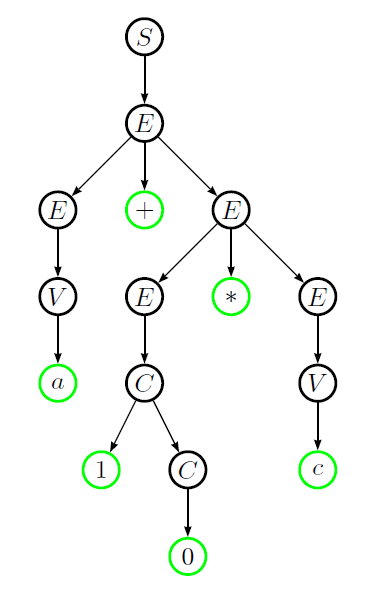
\includegraphics[width=6cm]{img/bez1}
			\end{figure}
\end{priklad}

\begin{veta}
Pokud $X \Rightarrow_{G,l}^* x$ pak existuje derivační strom $x$ z $X$ podle $G$.
\end{veta}


\begin{veta}
Pokud existuje derivační strom $x$ z $X$ podle $G$, pak $X \Rightarrow_{G,l}^* x$
\end{veta}


\begin{veta}
$S\Rightarrow_{G,l}^* u$ právě když existuje derivační strom $u$ z $S$ podle $G$.
\end{veta}

\subsubsection{Jednoznačné a nejednoznačné bezkontextové gramatiky}

\begin{definice}
Bezkontextová gramatika $G = \langle N,\Sigma,P,S \rangle$ se nazývá nejednoznačná, pokud existuje věta $x \in L(G)$, která má více než jeden derivační strom z $S$ podle $G$. V opačném případě se nazývá jednoznačná bezkontextová gramatika.
\end{definice}

\begin{definice}
Bezkontextový jazyk $L$ se nazývá jednoznačný pokud existuje jednoznačná gramatika $G$ tak, že $L=L(G)$.
\end{definice}

\begin{definice}
Bezkontextový jazyk $L$ se nazývá \textit{inherentně} nejednoznačný, pokud neexistuje žádná jednoznačná gramatika $G$ taková, že $L=L(G)$.
\end{definice}

\begin{veta}
Každý regulární jazyk je jednoznačný.
\end{veta}





\begin{priklad}
$L=\lbrace a^nb^nc^pd^p\ |\ n,p\ge 0\rbrace$ je inherentně nejednoznačný.
\end{priklad}

\subsection{Uzávěrové vlastnosti bezkontextových jazyků}

\begin{itemize}
\item
\textit{Sjednocení}

Mějme dány bezkontextové jazyky $L_1$, $L_2$ a korespondující bezkontexotvé gramatiky $G_1$ a $G_2$. Lze předpokládat, že množiny stavů obou gramatik jsou disjunktní (tj. $N_1 \cap N_2 = \emptyset$).

Dále uvažujeme gramatiku $G = \langle N,\Sigma,P,S \rangle$, kde \\
$N=N_1 \cup N_2 \cup \lbrace S \rbrace \\
\Sigma = \Sigma_1 \cup \Sigma_2 \\
P = P_1 \cup P_2 \cup \lbrace S \rightarrow S_1\ |\ S_2 \rbrace$

Platí, že $L(G)=L(G_1) \cup L(G_2)$.

\item
\textit{Produkt}

$L_1$ a $L_2$ jsou bezkontextové jazyky, $G_1$ a $G_2$ jsou odpovídající bezkontextové gramatiky.

Zavedeme gramatiku $G = \langle N,\Sigma,P,S \rangle$, kde \\
$N=N_1 \cup N_2 \cup \lbrace S \rbrace \\
\Sigma = \Sigma_1 \cup \Sigma_2 \\
P = P_1 \cup P_2 \cup \lbrace S \rightarrow S_1S_2 \rbrace$

Platí, že $L(G) = L(G_1) \cdot L(G_2)$.

\item
\textit{Kleeneho uzávěr}

Mějme bezkontextový jazyk $L$ a k němu odpovídající gramatiku $G$.

Vytvoříme novou gramatiku $G' = \langle N \cup \lbrace S' \rbrace,\Sigma,P \cup \lbrace S' \rightarrow \varepsilon\ |\ SS'\rbrace,S' \rangle$.

\item
\textit{Pozitivní uzávěr}

Podobné jako u Kleeneho uzávěru, akorát výsledná gramatika se bude lišit v množině pravidel.

$G' = \langle N \cup \lbrace S' \rbrace,\Sigma,P \cup \lbrace S' \rightarrow S\ |\ SS'\rbrace,S' \rangle$

\item
\textit{Průnik}

$\mathcal{L}_2$ není uzavřená na průnik.

\begin{priklad}
Uvedeme si příklad, který nám tvrzení potvrdí.\\
$\Sigma = \lbrace a,b,c \rbrace \\
L_1 = \lbrace a^nb^nc^*\ |\ n \ge 0 \rbrace \\
L_2 = \lbrace a^*b^nc^n\ |\ n \ge 0 \rbrace \\
\\
L_1 \cap L_2 = \lbrace a^nb^nc^n\ |\ n \ge 0 \rbrace$
\end{priklad}
Z toho také plyne, že není uzavřená ani na Komplement či Množinový rozdíl (De Morganovy zákony).
\end{itemize}

\paragraph{Bezkontextové gramatiky v programátorské praxi}

\textit{BNF}(Backus-Naurova forma):
Vytvořili ji John Backus a Peter Naur. Zápis se řidí několika pravidly:
\begin{itemize}
\item
neterminální symboly se zapisují do $\langle \ldots \rangle$
\item
používá se $::=$ místo $\rightarrow$
\item
terminální symboly se píší do uvozovek ($"*"$)
\item
pravidla se oddělují pomocí $|$
\end{itemize}

\begin{priklad}
Uvedeme si příklad zápisu gramatiky pomocí BNF.

$\langle expr \rangle ::= "(" \langle expr \rangle ")"\ |\ \langle expr \rangle\langle op \rangle\langle expr \rangle\ |\ \langle number \rangle \\
\langle op \rangle ::= "+"\ |\ "-"\ |\ "*"\ |\ "/" \\
\langle number \rangle ::= \langle digit \rangle \langle number \rangle\ |\ \langle digit \rangle \\
\langle digit \rangle ::= "0"\ |\ \ldots\ |\ "9"$
\end{priklad}

\textit{Extended BNF}: Zavedl Niklaus Wirth v roce 1977. Odpovídá BNF, pouze zjednodušuje její notaci a to tak že:
\begin{itemize}
\item
každé pravidlo je ukončeno znakem $";"$
\item
terminální symboly se píší do uvozovek, neterminální ne
\item
$[,]$ značí volitelnou část výrazu
\item
$\lbrace,\rbrace$ indukují možnost opakování
\item
$(,)$ jsou použity pro shlukování výrazů
\item
místo $::=$ se používá $=$
\item
terminální a neterminální symboly se oddělují čárkou
\end{itemize}

\begin{priklad}
Gramatiku z předchozího příkladu můžeme zapsat pomocí EBNF takto:

$expr="(",expr,")"\ |\ expr,op,expr\ |\ number;\\
op="+"\ |\ "+"\ |\ "-"\ |\ "*"\ |\ "/";\\
number=[signum],digit,\lbrace digit \rbrace;\\
digit="0"\ |\ \ldots \ |\ "9";\\
signum="+"\ |\ "-";$
\end{priklad}

	\subsection{Zásobníkové automaty a jejich modifikace}

\subsubsection{Nedeterministický zásobníkový automat}
Hledáme silnější analytický aparát, než jsou KDA, protože ty v určitých situacích selhávají.

\begin{priklad}
Mějme jazyk
$$L = \lbrace x \in \Sigma^{*}| \quad x \text{ je korektně uzávorkovaný výraz} \rbrace$$
Následně podrobněji
$$L = \lbrace x \in \Sigma^{*}| \Sigma = \lbrace (,),[,] \rbrace \quad x \text{ je korektně uzávorkovaný výraz} \rbrace$$
Do tohoto jazyka patří například řetězce $()[], ([]), \ldots$, ale nepatří do něj řetězce $()), ][][, \ldots$
\end{priklad}

\begin{figure}[H]
\centering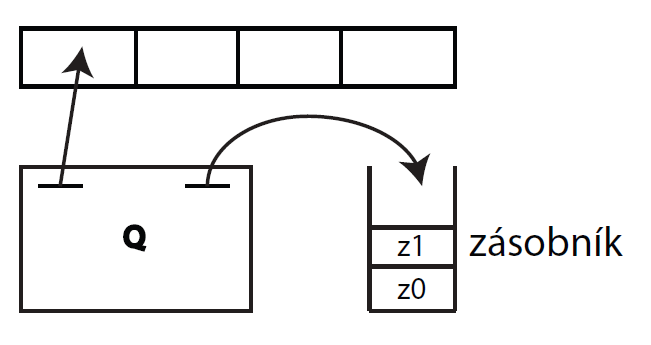
\includegraphics[width=7cm]{img/ZA}
\caption{Náčrt zásobníkového automatu.}
\end{figure}

\begin{definice}
Jako \textit{nedeterministický zásobníkový automat} označme následující strukturu:
$$
A = \langle \Sigma, \Gamma, Q, \delta, q_0, z_0, F \rangle
$$
Nyní si popišme význam nám dosud neznámých prvků tohoto automatu:
\begin{eqnarray*}
\Gamma &-& \text{ abeceda zásobnákových symbolů.} \\
z_0 &-& \text{ počáteční zásobníkový symbol.} \\
Q &-& \text{ konečná množina stavů.} \\
\delta &-& \text{ přechodová funkce ve tvaru } \delta : Q \times (\Sigma \cup \lbrace \varepsilon \rbrace) \times \Gamma \rightarrow 2^{Q \times \Gamma^{*}}
\end{eqnarray*}
Navíc $\langle \sigma, abc \rangle \in \delta(q, a, d)$ znamená slovně: \uv{Ze stavu $q$ po přečtení $a$ ze vstupu a symbolu $d$ ze zásobníku
 přejde automat $A$ do stavu $\sigma$ a na zásobník zapíše řetězec $"abc"$.} Mějme na paměti, že tento řetězec je na zásobník zapsán \uv{obráceně}.
\end{definice}

\begin{figure}[ht]
\centering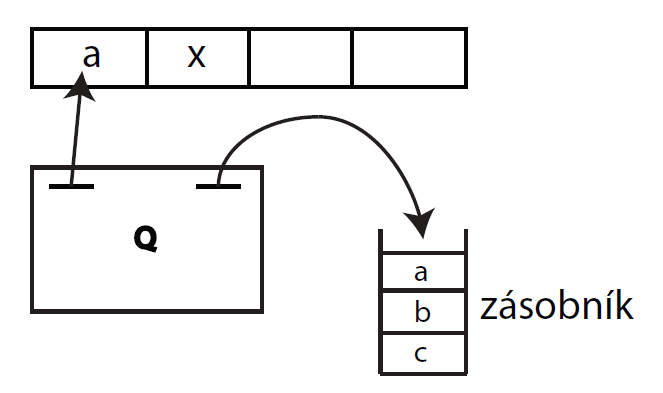
\includegraphics[width=7cm]{img/ZA2}
\caption{Vkládání hodnot na zásobník u NZA.}
\end{figure}

\subsubsection{Reprezentace NZA}

\paragraph{Přechodová tabulka}
V přechodové tabulce řádky odpovídají stavům a sloupce odpovídají prvkům $(\Sigma \cup \lbrace \varepsilon \rbrace) \times \Gamma$.
\begin{priklad}
\begin{eqnarray*}
Q &=& \lbrace q_0, q_1 \rbrace \\
\Sigma &=& \lbrace a, b \rbrace \\
\Gamma &=& \lbrace 0, 1 \rbrace
\end{eqnarray*}
\begin{table}[h]
\begin{center}
\begin{tabular}{ r || c | c | c | c | c | c}                   
 & $\langle a, 0 \rangle$ & $\langle b, 0 \rangle$ & $\langle c, 0 \rangle$ & $\langle a, 1 \rangle$ & $\langle b, 1 \rangle$ & $\langle c, 1 \rangle$ \\
\hline
$\rightarrow q_0^{\cdot}$ & $\cdots$ & $\cdots$ & $\cdots$ & $\cdots$ & $\cdots$ & $\cdots$ \\
$q_1^{\cdot}$ & $\cdots$ & $\lbrace \langle r, w \rangle \rbrace$ & $\cdots$ & $\cdots$ & $\cdots$ & $\cdots$
\end{tabular}
\end{center}
\caption{Ukázka přechodové tabulky pro NZA}
\end{table}
\end{priklad}

\paragraph{Přechodový diagram}
Přechodov\'e diagramy NZA jsou velmi podobn\'e diagramům KA.
\begin{center}
\begin{figure}[H]
\centering
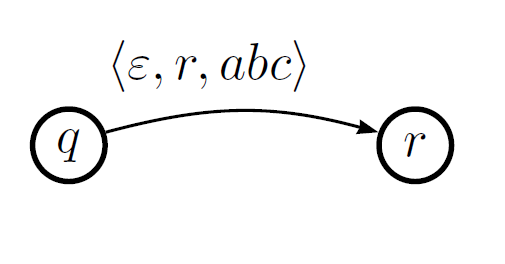
\includegraphics[width=7cm]{img/ZA3}
\end{figure}
\end{center}

\begin{definice}
Konfigurac\'i NZA je každ\'y prvek z množiny $Q \times \Sigma^* \times \Gamma^*$, tedy
$\langle q, abc, 001 \rangle \in Q \times \Sigma^* \times \Gamma^*$ znamená, že NZA je ve stavu $q$, na vstupu
zbývá přečíst řetězec \uv{abc} a na zásobníku je řetězec \uv{001}.

Pro konfigurace $\langle q_i, w_i, x_i \rangle \text{ a } \langle q_j, w_j, x_j \rangle$ klademe 
$\langle q_i, w_i, x_i \rangle \vdash \langle q_j, w_j, x_j \rangle$ právě, když platí:
\begin{itemize}
\item
$x_i = zy \text{ ,kde } z \in \Gamma, y \in \Gamma^*$

\item
$w_i = aw_j \text{ ,kde } a \in (\Sigma \cup \lbrace \varepsilon \rbrace), w_j \in \Sigma^*$

\item
$\langle q_j, x \rangle \in \delta(q_i, a, z)$
\end{itemize}
Přičemž $x_j = xy$.
\end{definice}

Reflexivní a tranzitivní uzávěr $\vdash$ označíme $\vdash^*$ a platí:
\begin{gather*}
\langle q_i, w_i, x_i \rangle \vdash^* \langle q_j, w_j, x_j \rangle \text{ právě, když} \\
\langle q_i, w_i, x_i \rangle \vdash \cdots \vdash \langle q_j, w_j, x_j \rangle
\end{gather*}
Pokud $\langle q_i, w_i, x_i \rangle \vdash^* \langle q_j, w_j, x_j \rangle$ tak říkáme, že existuje výpočet
NZA, kterým přejde tento NZA z $\langle q_i, w_i, x_i \rangle \text{ do } \langle q_j, w_j, x_j \rangle$.

\subsubsection{Jazyky rozpoznávané NZA}
\begin{enumerate}
\item
Jazyk rozpoznávaný pomocí koncových stavů automatu, tedy:
$$
L(A) = \lbrace w \in \Sigma^* | \quad \langle q_0, w, z_0 \rangle \vdash^* \langle q, \varepsilon, x \rangle, q \in F, x \in \Gamma^* \rbrace
$$

\item
Jazyk rozpoznávaný vyprazdňováním zásobníků, tedy:
$$
N(A) = \lbrace w \in \Sigma^* | \quad \langle q_0, w, z_0 \rangle \vdash^* \langle q, \varepsilon, \varepsilon \rangle, q \in Q \rbrace
$$
\end{enumerate}

\subsubsection{Rozpoznání jazyk způsobem přechodu od koncových stavů k vyprázdnění zásobníku}
\begin{veta}
Ke každému NZA $A$ existuje NZA $A'$, pro který platí $L(A) = N(A') = L(A')$
\end{veta}


Uvažujme
$$
A' = \langle \Sigma, \Gamma \cup \lbrace z_{0}' \rbrace, Q \cup \lbrace q_{0}', q_{\#}' \rbrace, \delta',
q_0', z_0', \lbrace q_{\#}' \rbrace \rangle
$$
kde $\delta'$ je přechodová funkce, jež vznikne rozšířením původní přechodové funkce o následující přechody:
\begin{gather*}
\delta'(q_0', \varepsilon, z_0') = \lbrace \langle q_0, z_0, z_0' \rangle \rbrace \\
\delta'(q, \varepsilon, z) = \delta(q, \varepsilon, z) \cup \lbrace \langle q_{\#}', \varepsilon \rangle \rbrace \text { pokud }
q \in F, a \in \Gamma \cup \lbrace z_0' \rbrace \\
\delta'(q_{\#}', \varepsilon, z) = \lbrace \rangle q_{\#}', \varepsilon \langle \rbrace \text{ pro } z \in \Gamma \cup \lbrace z_0' \rbrace
\end{gather*}

\subsubsection{Rozpoznání jazyk způsobem přechodu od vyprázdnění zásobníku k přijímání koncovými stavy}
\begin{veta}
Ke každému NZA $A = \langle \Sigma, \Gamma, Q, \delta, q_0, z_0, F \rangle$ existuje NZA $A'$ tak, že $N(A) = L(A') = N(A')$.
\end{veta}


\subsubsection{Automaty pracující s celým zásobníkem}
Pro automat pracující s celým zásobníkem má platit, že $\delta : Q \times (\Sigma \cup \lbrace \varepsilon \rbrace) \times \Gamma^*
 \rightarrow 2^{Q \times \Gamma^*}$ s omezením, že přechodová funkce je pro každé $q \in Q, a \in (\Sigma \cup \lbrace \varepsilon \rbrace)$ definována
pouze pro konečně mnoho řetězců $z \in \Gamma^*$ a navíc musí platit, že pro každý z konečně mnoha řetězců je $\delta(q, a, z)$ konečná.

Platí také:
$$
\langle q_i, w_i, z_i \rangle \vdash \langle q_j, w_j, z_j \rangle
$$
\begin{enumerate}
\item
$z_i = zy, z \in \Gamma^*, y \in \Gamma^*$

\item
$w_i = aw_j, a \in (\Sigma \cup \lbrace \varepsilon \rbrace)$

\item
$\langle q_j, x \rangle \in \delta(q_i, a, z)$

\item
$z_j = xy$
\end{enumerate}

\begin{veta}
Pro každý NZA $A$ pracující s celým zásobníkem existuje NZA $A'$ pracující pouze s vrcholem zásobníku.
\end{veta}

\begin{dusledek}
Třídy automatu jsou ekvivalentní.
\end{dusledek}

\subsubsection{Poznámky o vlastnostech NZA}

\begin{enumerate}
\item 
Pokud $\langle q,u,x \rangle \vdash^* \langle p,v,y \rangle$ pak $\langle q,uw,x \rangle \vdash^* \langle p,vw,y \rangle$ pro libovolný řetězec $w \in \Sigma^*$.

\item
Pokud $\langle q,u,x \rangle \vdash^* \langle p,v,y \rangle$ pak $\langle q,u,xz \rangle \vdash^* \langle p,v,yz \rangle$ pro libovolný řetězec $w \in \Gamma^*$.

\item
Pokud $\langle q,uw,x \rangle \vdash^* \langle p,vw,y \rangle$ pak $\langle q,u,x \rangle \vdash^* \langle p,v,y \rangle$.

\item[1.+2.]
Pokud $\langle q,u,x \rangle \vdash^* \langle p,v,y \rangle$ pak $\langle q,uw,xz \rangle \vdash^* \langle p,vw,yz \rangle$ pro všechny řetězce $w \in \Sigma^* $ a $z \in \Gamma^*$.

\item[1.+3.]
$\langle q,u,x \rangle \vdash^* \langle p,v,y \rangle$ právě když $\langle q,uw,x \rangle \vdash^* \langle p,vw,y \rangle$.
\end{enumerate}

\begin{poznamka}
Opak 2. vlastnosti neplatí: Pokud $\langle q,u,xz \rangle \vdash^* \langle p,v,yz \rangle$ pak obecně nelze odvodit, že $\langle q,u,x \rangle \vdash^* \langle p,v,y \rangle$.\\
Speciálně: $x=y=\varepsilon$
\end{poznamka}

\begin{poznamka}
$\langle q,u,z \rangle \vdash^* \langle p,\varepsilon,\varepsilon \rangle$: automat je schopen přejít ze stavu $q$ do $p$, přitom zkonzumuje řetězec $u$ ze vstupu a řetězec $z$ ze zásobníku, ale bez toho, aniž by se někdy během činnosti dostal pod úroveň řetězce $z$ na zásobníku.
\end{poznamka}

	\subsection{Deterministické zásobníkové automaty, Deterministické bezkontextové jazyky}

	
\begin{definice}
Řekneme, že zásobníkový automat $A = \langle \Sigma,\Gamma,Q,\delta,q_0,z_0,F \rangle$ je \textit{deterministický} (DZA), pokud jsou pro každé $q \in Q$ a $z \in \Gamma$ splněny následující podmínky:
\begin{enumerate}
\item
pro všechny $a \in \Sigma \cup \lbrace \varepsilon \rbrace$ platí $|\delta (q,a,z)| \le 1$
\item
pokud $\delta (q,\varepsilon,z) \neq \emptyset$ pak $\delta (q,a,z) = \emptyset$ pro každé $a \in \Sigma$
\end{enumerate}
\end{definice}

Nabízí se otázka, jaké třídy jazyků, jsou vlastně rozpoznatelné deterministickým zásobníkový automatem pomocí buď koncových stavů, nebo vyprázdněním zásobníku.

\begin{definice}
Bezkontextový jazyk $L$ se nazývá \textit{deterministický}, pokud existuje deterministický zásobníkový automat $A$ tak, že $L = L(A)$.
\end{definice}

\begin{definice}
Bezkontextový jazyk $L$ má \textit{prefixovou vlastnost}, pokud $L$ neobsahuje dva různé řetězce $x,y$ tak, že $x$ je prefixem $y$.
\end{definice}

\begin{veta}
Pro libovolný bezkontextový jazyk $L$ jsou následující tvrzení ekvivalentní:
\begin{enumerate}
\item
$L = N(A)$ pro nějaký DZA $A$
\item
$L = L(A')$ pro nějaký DZA $A'$ a $L$ má prefixovou vlastnost
\end{enumerate}
\end{veta}



\begin{dusledek}
Deterministický bezkontextový jazyk má prefixovou vlastnost, právě když je přijímán nějakým DZA pomocí vyprázdnění zásobníku.
\end{dusledek}

\begin{veta}
Každý regulární jazyk je deterministický.
\end{veta}


\begin{priklad}
Následující jazyk je deterministický:
$$
L = \lbrace a^nb^n\ |\ n\ge1 \rbrace
$$
\end{priklad}

\begin{poznamka}
Mnoho regulárních jazyků \textit{nemá} prefixovou vlastnost.
\end{poznamka}

\begin{veta}
Pokud $L=N(A)$ pro DZA $A$, pak je $L$ jednoznačný.
\end{veta}



\begin{veta}
Pokud $L=L(A)$ pro DZA $A$, pak je $L$ jednoznačný. Deterministické bezkontextové jazyky jsou jednoznačné.
\end{veta}


%============================================================================
%                                                                             DRUHÝ ODSTAVEC
%============================================================================

\section{Druhý odstavec}

Turingův stroj (TS), nedeterministický TS. Jazyk přijímaný TS, jazyk rozhodovaný TS. Church-Turingova
teze, varianty TS. Částečně rekurzivní a rekurzivní jazyky, jazyky a rozhodovací problémy. Vztah rekurzivních
a částečně rekurzivních jazyků. Uzávěrové vlastnosti jazyků TS. Riceova věta. Vztah jazyků TS k jazykům
Chomského hierarchie. Věta o rekurzi.

	\subsection{Turingův stroj (TS)}

		\begin{itemize}
			\item Alan Turing, 1936
			\item účel: porozumět omezením mechanického výpočtu
		\end{itemize}
		\textbf{TS se skládá z}
		\begin{itemize}
			\item řídící jednotky, která se vždy nachází v jednom z konečného množství stavů
			\item zleva omezené nekonečné pásky rozdělené na políčka, v každém políčku je zapsán jeden symbol
			\item čtecí / zapisovací hlavy která je vždy umístěna nad jedním políčkem pásky
		\end{itemize}
		\textbf{Definice: }
		Turingův stroj je struktura $\langle Q, \Sigma, \Gamma, \delta, q_{start}, q_{+}, q_{-} \rangle $ dána:
		\begin{itemize}
			\item Neprázdnou konečnou množinou stavů $Q$
			\item Vstupní abecedou  $\Sigma$ t.ž. \textvisiblespace $ \notin \Sigma$
			\item páskovou abecedou $\Gamma$ t.ž. $\Sigma \subset \Gamma,$ \textvisiblespace $\in  \Gamma $
			\item přechodovou funkcí $\delta : Q \times  \Gamma \rightarrow Q \times \Gamma \times \{L , R \} $
			\item počátečním stavem $q_{start} \in Q$
			\item přijímacím stavem $q_{+} \in Q $ a zamítacím stavem $q_{-} \in Q.$ $q_{+} \neq q_{-}$
		\end{itemize}
		Program TS lze chápat jako množinu elementárních instrukcí ve tvaru:

		\textit{\uv{Pokud je řídící jednotka ve stavu $q$ a čtecí/zapisovací hlava čte symbol $a$, tak změň stav řídící jednotky
		na $q'$, na pásku zapiš $a'$ a posuň
		čtecí/zapisovací hlavu o jedno políčko směrem $d$.}}

		Takováto instrukce se zapisuje jako $\delta (q,a) = (q', a', d)$ a nazýváme ji přechod. Celý program, tedy množinu 				takovýchto instrukcí, pak nazýváme přechodovou funkcí TS

		\textbf{Konfigurace} TS je uspořádaná trojice $(q, \alpha, n) \in Q \times \Gamma^{*} \times N_{0}$ , která zachycuje
		aktuální status všech tří komponent.
		\begin{itemize}
			\item $q$ je aktuální stav řídící jednotky
			\item $\alpha$ je obsah pásky
			\item $n$ je pozice hlavy
		\end{itemize}

		\textbf{Krok výpočtu TS} je definován jako binární relace na množině konfigurací: Nechť $(q,a_{0} \dots a_{n}, i) $
		je taková konfigurace $T$, kde $q \neq q_{\pm}, n \in N_{0}, a_{0}, \dots, a_{n}~\in~\Gamma, i~\leq~n. $
		\begin{itemize}
			\item Je-li $1 \leq i \leq n a \delta(q,a_{i}) = (q', b, L), pak$
				$$(q,a_{0} \dots a_{n}, i) \vdash (q', a_{0} \dots a_{i-1}ba_{i+1} \dots a_{n}, i-1) $$
			\item Je-li $\delta(q,a_{0}) = (q', b, L), pak$
				$$(q,a_{0} \dots a_{n}, 0) \vdash (q', ba_{1} \dots a_{n}, 0) $$
			\item Je-li $\delta(q,a_{i}) = (q', b, R), pak$
				$$(q,a_{0} \dots a_{n}, i) \vdash (q', a_{0} \dots a_{i-1}ba_{i+1} \dots a_{n}, i+1) $$
		\end{itemize}



	\subsection{Nedeterministický TS}

		Obdobný rozdíl jako u konečných deterministických a konečných nedeterministických automatů. Přechodová funkce ve 				tvaru:
		$$\delta : Q \times  \Gamma \rightarrow 2^{Q \times \Gamma \times \{L , R \}}$$

		\textbf{Definice: }
		Nedeterministický TS je struktura $\langle Q, \Sigma, \Gamma, \delta, q_{start}, q_{+}, q_{-} \rangle $ dána:
		\begin{itemize}
			\item Neprázdnou konečnou množinou stavů $Q$
			\item Vstupní abecedou  $\Sigma$ t.ž. \textvisiblespace $ \notin \Sigma$
			\item páskovou abecedou $\Gamma$ t.ž. $\Sigma \subset \Gamma,$ \textvisiblespace $\in  \Gamma $
			\item přechodovou funkcí $\delta : Q \times  \Gamma \rightarrow 2^{Q \times \Gamma \times \{L , R \}} $
			\item počátečním stavem $q_{start} \in Q$
			\item přijímacím stavem $q_{+} \in Q $ a zamítacím stavem $q_{-} \in Q.$ $q_{+} \neq q_{-}$
		\end{itemize}

		Ke každému deterministickému existuje ekvivalentní nedeterministický automat a ke každému
		nedeterministickému existuje ekvivalentní deterministický automat.

	\subsection{Jazyk přijímaný TS}

		Množinu všech slov $\omega \in \Sigma^{*}$, které TS \textit{T} Přijímá značíme \textit{L(T)} a nazýváme 					\textit{\textbf{jazykem Turingova stroje}}, t.j.
		 $$L(T) = \{ \omega | \omega \in \Sigma^{*}, (\omega, q_{0},0) \vdash^{*} C_{+}\} $$
		Jazyk $L(T)$ nazýváme \textit{jazyk přijímaný TS} $T$.\\
		Říkáme, že TS $T$ \textit{přijímá jazyk}$ L(T)$.\\

		Jazyk $L \subseteq \Sigma^{*} $ nazveme\textit{ jazyk přijímaný TS}, pokud existuje TS $T$ který jej přijímá.

	\subsection{Jazyk rozhodovaný TS}

		Pokud navíc platí, že TS $T$ zamítá každé $\omega \notin L(T)$, nazýváme jazyk L(T)
		\textit{jazyk~rozhodovaný} TS $T$.\\
		Říkáme, že TS $T$ \textit{rozhoduje jazyk} $L(T)$. (to znamená že nikdy necyklí)

		Jazyk $L \subseteq \Sigma^{*} $ nazveme\textit{ jazyk rozhodovaný TS}, pokud existuje TS $T$ který jej rozhoduje.


	\subsection{Churg-Turingova teze}

		\textit{Intuitivní pojem algoritmu = algoritmus TS.} \\(to je všechno co k tomu máme)

	\paragraph{Wikipedie:}
	Teze může znít například takto: \textit{\uv{Ke každému algoritmu existuje ekvivalentní Turingův stroj.}}
Kvůli neformální definici pojmu algoritmus nemůže být tato teze nikdy dokázána, lze ji ale vyvrátit, podaří-li se sestrojit stroj, který bude umět řešit problémy, které Turingův stroj řešit neumí (např. problém zastavení).

Jelikož každý počítačový program lze přeložit do jazyka Turingova stroje a obvykle i naopak, lze tezi ekvivalentně formulovat pro kterýkoli běžně používaný programovací jazyk. Přesněji, programovací jazyk potřebuje jednu z následujících konstrukcí (kromě jiných), aby byl turingovsky úplný (tj. ekvivalentní Turingovu stroji):

		\begin{itemize}
			\item cyklus while-do
			\item neomezenou (alespoň teoreticky) rekurzi
			\item podmíněný skok
		\end{itemize}
Běžné programovací jazyky mívají všechny tři tyto konstrukce. Mezi jazyky, které turingovsky úplné nejsou, patří SQL (myšleno bez vložených procedur) a Charity.

	\subsection{Varianty TS}
		\begin{itemize}
			\item TS, který se nikdy nepokusí přejet levý okraj pásky
				\begin{itemize}
					\item Rozumíme TS, u kterého při výpočtu nad jakýmkoli slovem nedojde k tomu že, je v konfiguraci
						$(q,a\omega,0)$ a existuje přechod $\delta(q,a) = (q',b,L).$  Tedy nikdy nenastane situace
						že by byla hlava nad nejlevějším políčkem pásky a přechodová funkce by určovala pohyb 								vlevo.
				\end{itemize}
			\item TS, který nikdy nezapíše na pásku \textvisiblespace
				\begin{itemize}
					\item Roziníme TS, který nemá žádný přechod ve tvaru $\delta(q,a) = (q',$ \textvisiblespace $,D)$
				\end{itemize}
			\item TS, který \uv{ po sobě uklízí}
				\begin{itemize}
					\item Roziníme TS, který zastaví pouze v konfiguraci $\langle q_{+}, \epsilon, 0 \rangle$
						nebo $\langle q_{-}, \epsilon, 0 \rangle$. Tzn. smaže obsah pásky.
				\end{itemize}
			\item ( předchozí 3 se nejspíš nepočítají mezi varianty TS)
			\item \textbf{TS s instrukcí stop} --- struktura  $\langle Q, \Sigma, \Gamma, \delta, q_{start}, q_{+}, q_{-} \rangle $
								dána:
				\begin{itemize}
					\item Neprázdnou konečnou množinou stavů $Q$
					\item Vstupní abecedou  $\Sigma$ t.ž. \textvisiblespace $ \notin \Sigma$
					\item páskovou abecedou $\Gamma$ t.ž. $\Sigma \subset \Gamma,$ \textvisiblespace $\in  \Gamma $
					\item přechodovou funkcí $\delta : Q \times  \Gamma \rightarrow Q \times \Gamma \times \{L, S, R \} $
					\item počátečním stavem $q_{start} \in Q$
					\item přijímacím stavem $q_{+} \in Q $ a zamítacím stavem $q_{-} \in Q.$ $q_{+} \neq q_{-}$
				\end{itemize}
				Odpovídajícím způsobem se upraví definice kroku výpočtu, vlatně se přidá bod:

				-- Je-li $\delta(q, a_{i}) = (q', b, S)$, pak
					$$(q,a_{0} \dots a_{n}, i) \vdash (q', a_{0} \dots a_{i-1}ba_{i+1} \dots a_{n},i) $$
			\item \textbf{TS s oboustranně nekonečnou páskou} --- definice je totožná jako u klasického TS; rozdíl je v definici
			 konfigurace (nevystačíme si s $\langle q, \omega, i \rangle \in Q \times \Gamma^{*} \times N_{0}$)a výpočtu
			(není zarážení o levý okraj)
				\begin{itemize}
					\item \textbf{Konfigurace:} Alternativně zapisujeme jako řetězec
					 	$\alpha q\beta \in \Gamma^{*}Q\Gamma^{*}.$
						Konfigurace $\alpha q\beta$ představuje status stroje, který má na pásce zapsán řetězec
						$ \alpha\beta$,
						hlava	je nad prvním symbolem řetězce $\beta$, řídící jednotka je ve stavu q.

						U TS s oboustranně nekonečnou páskou považujeme $\alpha q\beta$ za totožnou s
						$\alpha q\beta$\textvisiblespace a s \textvisiblespace$\alpha q\beta$.
					\item \textbf{Krok výpočtu TS (s oboustranně nekonečnou páskou)} je definován jako binární
						relace na množině konfigurací: Nechť $\alpha aqb\beta$ je taková konfigurace $T$, kde
						$q \neq q, \alpha, \beta \in \Gamma^{*}, a,b \in \Gamma.$
						\begin{itemize}
							\item Je-li $\delta(q,a) = (q', x, L) $, pak  $$\alpha aqb\beta \vdash \alpha q'ax\beta$$.
							\item Je-li $\delta(q,a_{1}) = (q', x, R) $, pak
									$$\alpha aqb\beta \vdash \alpha axq'\beta$$.
						\end{itemize}
				\end{itemize}
					\item \textbf{TS s více páskami} --- je struktura $\langle Q, \Sigma, \Gamma, \delta, q_{0}, q_{+},
						q_{-} \rangle $ dána:
						\begin{itemize}
							\item Neprázdnou konečnou množinou stavů $Q$
							\item Vstupní abecedou  $\Sigma$ t.ž. \textvisiblespace $ \notin \Sigma$
							\item páskovou abecedou $\Gamma$ t.ž. $\Sigma \subset \Gamma,$ \textvisiblespace
								$\in  \Gamma $
							\item přechodovou funkcí $\delta : Q \times  \Gamma^{k} \rightarrow Q \times [ \Gamma
								\times \{L, R \} ]^{k}$
							\item počátečním stavem $q_{start} \in Q$
							\item přijímacím stavem $q_{+} \in Q $ a zamítacím stavem $q_{-}
								\in Q.$ $q_{+} \neq q_{-}$
						\end{itemize}
					\item \textbf{Lineárně ohraničený TS (LBA)} --- klasický nedeterministický  TS ale na pásce se pohybuje jen mezi dvěma zarážkami které nikdy nepřejede a nepřepíše (jako TS který nikdy nepřejede levý okraj)

		\end{itemize}
		Ke každé variantě TS vždy existuje ekvilalentní klasický TS a obráceně.



	\subsection{Částečně rekurzivní a rekurzivní jazyky, Jazyky a rozhodovací problémy, Vztah rekurzivních a částečne rekurzivních jazyků }

		\begin{itemize}
			\item Jazykům rozhodovaným TS říkáme \textbf{rekurzivní jazyky (R)}
			\item Jazykům přijímaným TS říkáme \textbf{ částečně rekurzivní jazyky (ČR)}
			\item R $\subseteq$ ČR
		\end{itemize}


		\begin{figure}[!h]
		\centering
		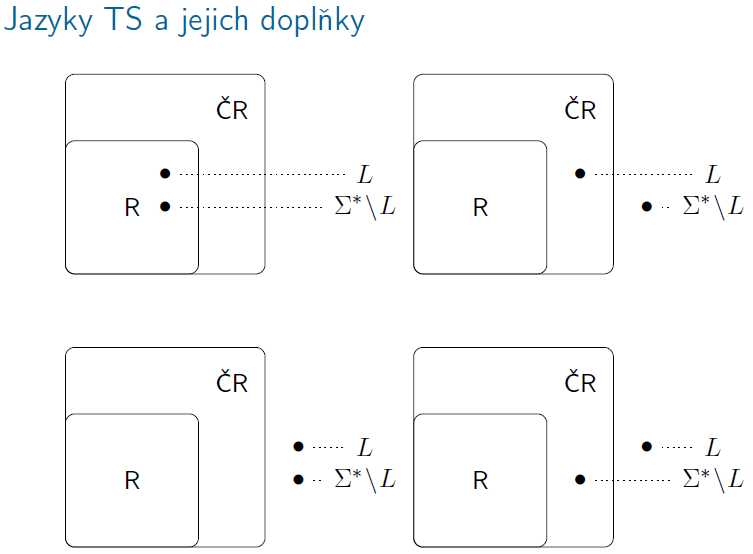
\includegraphics[width=12cm]{img/jazykyAJejichDoplnky}
		\caption{Jiné stavy nastat nemůžou !!!}
		\end{figure}

		\vspace{1cm}
		\textbf{Jazyky, které jsou částečně rekurzivní ale nejsou rekurzivní:}

		\begin{itemize}
			\item Univezální jazyl $L_{U}$ definován takto : $$L_{U} = \{ [T,w]| T \text{ je } TS \text{, který přijímá } w\}$$
			\item Jazyk $L_{\text{HALT}}$ definován takto:
						$$L_{\text{HALT}} = \{ [T,w]| T \text{ je } TS \text{, který zastaví pro } w\}$$
			\item Jazyk  $L_{\text{NE}}$ definován takto:
					$$L_{\text{NE}} = \{ [ T ] |  L(T)  \neq  \emptyset\} \text{\dots (zastaví alespoň pro jedno slovo)} $$

		\end{itemize}

		\textbf{Jazyky, které nejsou částečně rekurzivní:}

		\begin{itemize}
			\item Diagonální jazyk $L_{d}$ $$L_{d} = \{[T]| T \text{ je } TS \text{, který nepřijímá svůj kód} \}$$
			\item Jazyk strojů přijímajících prázdný jazyk
				$$L_{\emptyset} = \{[T]| T \text{ je } TS \text{ a } L(T) =
						\emptyset \} \text{\dots(všechny slova zamítne?)}$$
			\item Jazyk strojů, které se nezacyklí
				$$L_{noncycle} = \{ [T]| T \text{ je } TS \text{ a necyklí pro žádné slovo } w\}$$
		\end{itemize}

		\vspace{1cm}
		JAZYK $\approx$ PROBLÉM

		\begin{itemize}
			\item $L_{U} \rightarrow$ problém přijetí
			\item $L_{HALT} \rightarrow$ problém zastavení
			\item $L_{NE} \rightarrow$ problém neprázdnosti jazyka
		\end{itemize}
		\vspace{1cm}


	\subsection{Uzávěrové vlastnosti jazyků TS}

	\textbf{Věty:}
		\begin{itemize}
			\item Pokud $L$ je rekurzivní pak, $\Sigma^{*} \setminus  L$ je rekurzivní (staší sestrojit TS který rozhoduje L
				a prohodit přijímací a zamítací stavy).
			\item Nechť $L_{1}, L_{2} \in R$ jsou rekurzuvní jazyky, pak $L_{1} \cup L_{2} \in R$  a  $L_{1} \cap L_{2} \in R$.
			\item Nechť $L_{1},L_{2} \in R$, pak $L_{1} \circ  L_{2}\in R$
			\item Pokud $L \in R$, pak $L^{*} \in R$ \dots($L^{*}$ je kleenyho uzávěr- zřetězení slov z L)



			\item Nechť $L_{1}, L_{2} \in$ ČR pak:
				\begin{itemize}
					\item $L_{1} \cup L_{2} \in$ ČR
					\item $L_{1} \cap L_{2} \in$ ČR
					\item $L_{1} \circ L_{2} \in$ ČR
					\item $L^{*} \in $ ČR
				\end{itemize}
			\item Pokud $L \in $ ČR a  $\Sigma^{*} \setminus  L \in $ ČR, pak $L \in R$

		\end{itemize}

	\subsection{Riceova věta :}

	Nechť $L$ je jazyk, jehož slova jsou kódy TS, a platí:
	\begin{itemize}
		\item pokud $L(T_{1}) = L(T_{2})$, pak $[T_{1}] \in L \leftrightarrow [T_{2}] \in L $
		\item $\exists T_{1},T_{2}$ t.ž. $ [T_{1}] \in L, [T_{2}] \notin L$
	\end{itemize}
	pak L není rekurzivní.\\
	\vspace{0,5cm}

	\textit{\textbf{Věta slovně:} Pokud se rovnají jazyky strojů, pak jejich kódydo jazyku buďto oba
				patří nebo oba nepatří a dále existuje alespoň jeden stoj jehož kód do tohoto jazyka nepatří a
				 alespoň jeden který do něj patří, pak není rekurzivní. (zjevně vyplývá třetí podmínka že slova
				 těchto jazyků musí být kódy TS)}\\

	\vspace{0,5cm}

	Tvzdení ve tvaru implikace né ekvilalence! Tzn. že lze použít pouze k důkazu, že nějaký jazyk není rekurzivní a nelze použít
	k důkazu že nějaký jazyk je rekurzivní.


	\subsection{Vztah jazyků TS k jazykům Chomského hierarchie}

		\vspace{5mm}
		$$\text{Typ 3} \subset \text{Typ 2} \subset \text{Typ 1} \subset \text{R} \subset \text{Typ 0} = \text{ČR} $$
		\begin{itemize}
		\item regulární jazyky = jazyky KA
		\item bezkontextové jazyky = jazyky nedeterministických ZA
		\item kontextové jazyky = jazyky LBA (lineárně ohraničený TS)
		\item jazyky gen. gramatikami bez omezení = jazyky přijímané TS
		\end{itemize}


		\textbf{Věty: }
		\begin{itemize}
		\item Třídy jazyků generovaných gramatikami typu 0 = částečně rekurzivní jazyky.
		\item Jazyky generované kontextově závislými gramatikamy = jazyky přijímané LBA
		\item Existuje rekurzivní jazyk, který není generovaný kontextovou gramatikou.
		\end{itemize}

		\begin{figure}[!h]
		\centering
		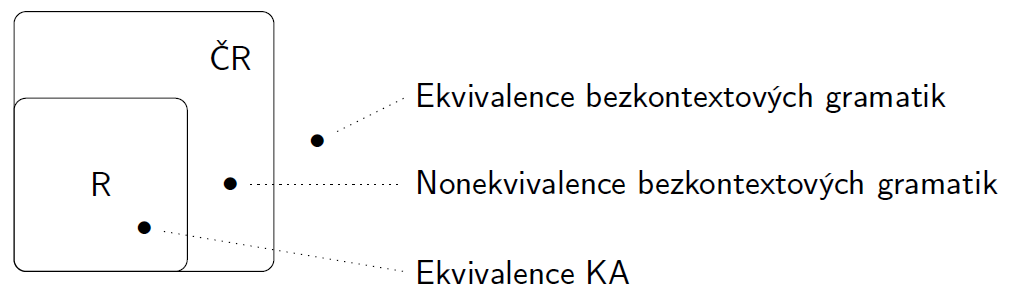
\includegraphics[width=8cm]{img/chomskyVSts}
		\end{figure}

	\subsection{Věta o rekurzi}

		TS \textit{vyčísluje funkci $f$}, pokud pro každé slovo $w \in \Sigma^{*}$ zapíše na pásku $f(w)$ a skončí.
		\vspace{5mm}

		\textbf{Věta o rekurzi: }Nechť $T$ je TS, který vyčísluje
			$t : \Sigma^{*} \times \Sigma^{*} \rightarrow \Sigma^{*}$. Existuje TS $R$, který
		počítá funkci $ r : \Sigma^{*} \rightarrow \Sigma^{*}$, kde pro každé $w$ platí $$r(w) = t(\langle R \rangle,w)$$

		\textit{Tvrzení věty říká, že abychom vytvořili TS $R$, který pracuje s vlastním kódem, stačí umět udělat
			 TS $T$, který pracuje stejně, ale dostává kód [R] na vstup. }\\

		\vspace{5mm}

		\begin{figure}[H]
			\centering
			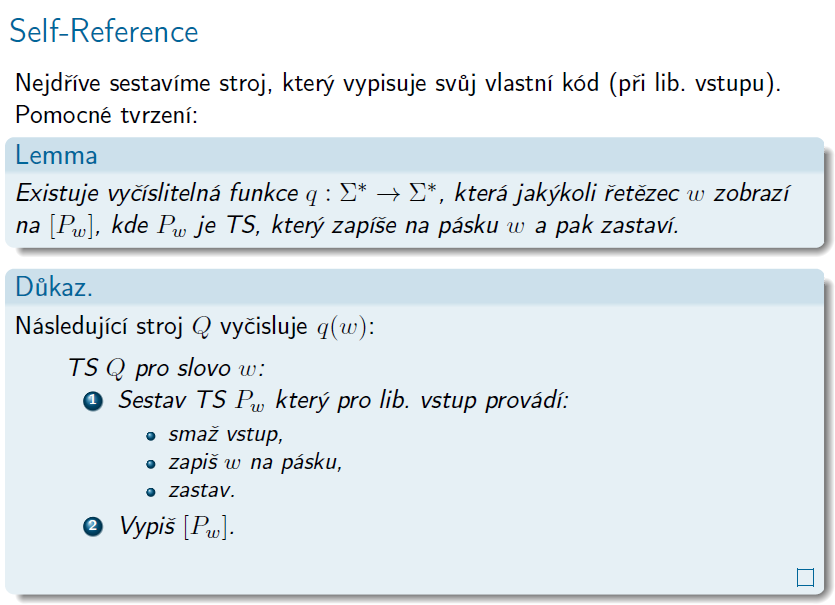
\includegraphics[width=15cm]{img/self1}
			\end{figure}

		\begin{figure}[H]
			\centering
			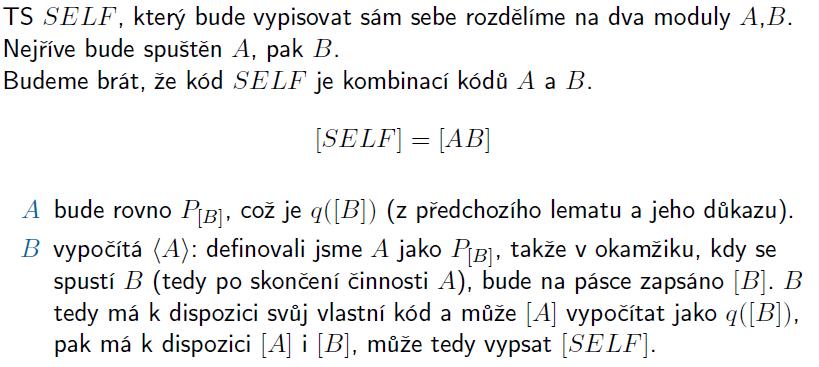
\includegraphics[width=15cm]{img/self2}
			\end{figure}

		\begin{figure}[H]
			\centering
			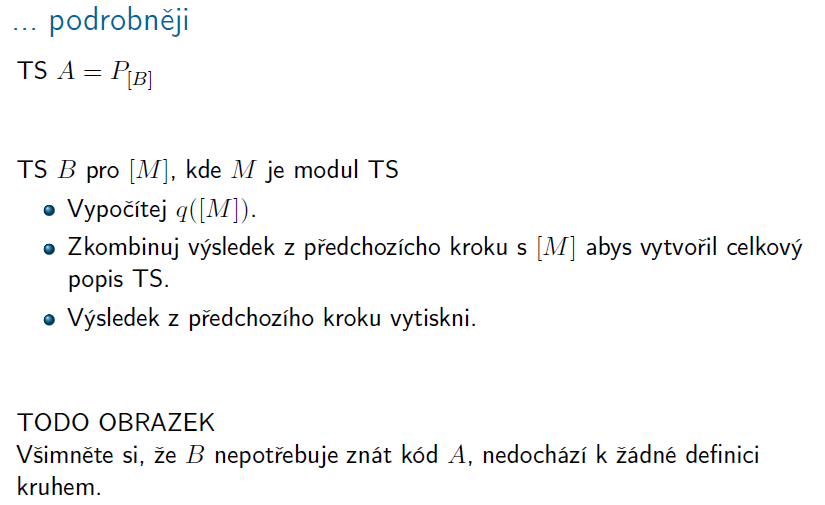
\includegraphics[width=15cm]{img/self3}
			\end{figure}

		\textbf{Aplikace věty o rekurzi -- Věta o pevném bodě:}
		Nechť $t : \Sigma^{*} \rightarrow \Sigma^{*}$ je vyčíslitelná funkce. Pak existuje TS $F$, t.ž. $t([F])$ je kód
		ekvivalentního TS.

%============================================================================
%                                                                             TŘETÍ ODSTAVEC
%============================================================================

\section{Třetí odstavec}

Složitost algoritmu (časová a paměťová). Třída P, třída NP, důvody jejich zavedení, jejich vzájemný vztah. NP-
úplné problémy. Cook-Levinova věta. Příklady NP-úplných problémů, dokazovaní NP-úplnosti. Třída PSPACE,
její vztah k třídám P a NP, PSPACE-úplné problémy. Třídy N a NL a NL-úplné problémy.

	\subsection{Složitost algoritmu(časová a paměťová)}

		\textbf{Časová složitost} = funkce $f : N \rightarrow N_{0}$, kde $f(n)$ je maximální
		počet kroků při výpočtu nad jakýmkoli vstupem délky $n$.\\
		\vspace{3mm}

		\textbf{Paměťová složitost} = funkce $f : N \rightarrow N$, kde $f(n)$ je maximální
		 počet políček při výpočtu nad jakýmkoli vstupem délky $n$.
		\\\vspace{3mm}

		$f,g : N \rightarrow R$\\
		$g(n)$ je \textbf{asymptotická hosní hranice} $f(n)$, když existují $c, n_{0} \in N$, t.ž. pro každé $n~\geq~n_{0}$:
		$$f(n) \leq c \cdot g(n)$$
		Notace: $f(n) = O(g(n))$


	\subsection{Třída P, NP, důvody jejich zavedení, vzájemný vztah}

		\textbf{turingův stroj}
		$$TIME(t(n)) = \{ L | L \text{rozhodovaný TS v čase} O(t(n))\}$$
		$$SPACE(s(n)) = \{ L | L \text{rozhodovaný TS v paměti} O(s(n))\}$$
		\vspace{3mm}
		\textbf{nedeterministický turingův stroj}

		NTS časová složitost t(n) \dots TS časová složitost $2^{O(t(n))}$\\

		NTS paměťová složitost t(n) \dots TS časová složitost $O(t^{2} (n))$

		$$NTIME(t(n)) = \{ L | L \text{rozhodovaný NTS v čase} O(t(n))\}$$
		$$NSPACE(s(n)) = \{ L | L \text{rozhodovaný NTS v paměti} O(s(n))\}$$\\

		\vspace{3mm}
		\textbf{Třídy P a NP:}
		$$P = \bigcup\{TIME(n^k) | k \in N\}$$
		$$NP = \bigcup\{NTIME(n^k) | k \in N\}$$
	\vspace{3mm}

	Víme že $$P\subseteq NP$$

	co ale nevíme je jestli $$NP\subseteq P \text{ tzn. (P=NP) nebo jestli } NP\nsubseteq P$$


	\subsection{NP--úplné problémy}

		Funkce $f :  \Sigma^{*} \rightarrow \Sigma^{*}$ je \textbf{funkce vyčíslitelná v polynomiálním čase}, pokud existuje TS
		pracující v polynomiálním čase, který pro každé $w \in  \Sigma^{*}$ zastaví a na pásce má zapsáno $w$.

		Jazyk A je \textbf{redukovatelný v polynomiálním čase} na jazyk B, načeno $A \leq_P B$, pokud existuje redukce
		v polynomiálním čase, tj. $r :  \Sigma^{*} \rightarrow \Sigma^{*}$, t.ž. $$w \in A \text{ p. k. } f(w) \in B$$

		\vspace{3mm}
		Jazyk B je \textbf{NP-úplný}, pokud
		\begin{itemize}
			\item B je v NP
			\item B je NP-těžký. Tj. pro každý $A\in NP$ platí $A\leq_P B$
		\end{itemize}

		\vspace{3mm}
		\textbf{Věty:}
		\begin{itemize}
			\item Pokud B je NP-úplný a $B \in P$, pak $P = NP$
			\item Pokud B je NP-úplný a $B \leq_P C$ pro $C \in $ NP, pak je NP-úplný
			\item SAT je NP-úplný
			\item 3SAT je NP-úplný
		\end{itemize}

		Hlavní důvod, proč jsou NP-úplné úlohy tak zajímavé, je právě jejich velmi obtížná řešitelnost. Díky ní nacházejí uplatnění v
 		moderní kryptografii, kde musíme být schopni rychle ověřovat správnost řešení, ale jeho nalezení musí trvat dlouho. Obtížnost
		výpočtu ovšem záleží i na konkrétních datech, pro speciální množinu vstupů může být úloha polynomiální, například řešíme-li
		obarvení třemi barvami pro jednoduché grafy (cesty).



	\subsection{Cook--Levinova věta}
		\textbf{Věta:} SAT je NP-úplný \dots (vic k tomu nemáme a důkaz psat nebudu stejně byste
			 se na to vysrali a mě už ten \LaTeX  pěkně mrdá)

		Na wikipedii je ta věta: \uv{Existuje NP-úplný problém}. Víc nic. 

	\subsection{Příklady NP--úplných problémů}
		\begin{itemize}
			\item SAT je NP-úplný
			\item 3SAT je NP-úplný
			\item  hledání  hamiltonovské kružnice v grafu
			\item vrcholové pokrytí
			\item trojrozměrné párování
		\end{itemize}

	\subsection{Dokazování NP--úplnosti}

		\textbf{Věta:} Pokud B je NP-úplný a $B \leq_P C$ pro $C \in $ NP, pak $C$ je NP-úplný

	\subsection{Třída PSPACE, její vztah k třídám P a NP}

		PSPACE je třída jazyku, které jsou rozhodnutelné v polynomickém čase na (deterministickém) TS, tedy
		$$\text{PSPACE} = \bigcup_k \text{SPACE}(n^k)$$
		\textit{(ve slajdech je napsáno v polynomickém čase, ale podle mě tam má být polynomická paměť)}\\
		Ze Savitchovy věty plyne že $$\text{PSPACE} = \text{NPSPACE}$$
		Celkově tedy máme:
		$$\text{ P } \subseteq \text{ NP } \subseteq \text{ PSPACE } \subseteq \text{ EXPTIME } $$  kde
		$\text{EXPTIME} = \bigcup_k \text{TIME}(2^n)$\\
		Alespoň jedna z těchto inkluzí je vlastní: ví se, že P~$\neq$~EXPTIME.\\
		Věří se, že všechny ty jsou vlastní.


	\subsection{PSPACE--úplné problémy}

		Jazyk $B$ je \textbf{PSPACE-úplný problém}, pokud
		\begin{itemize}
			\item $B \in$ PSPACE
			\item $B$ je PSPACE-těžký, tj. každý $A \in$ PSPACE je redukovatelný v polynomickém čase na $B$
		\end{itemize}\vspace{3mm}
		\textbf{Grafová hra:} Mějme orientovaný graf G s vyznačeným počátečním uzlem $u_1$
		\begin{itemize}
			\item Aktuální uzel je na začátku $u_1$
			\item Hráči se střídají v tazích
			\item Hráč na tahu zvolí souseda $u_1$, ten se stává aktuálním uzlem, nelze vybrat uzel, který už byl předtím
				navštíven
			\item Hráč, který uvízne prohrává
		\end{itemize}
		$$GG = \{[G,b] | \text{ hráč 1 má vítěznou strategii pro G a poč. b } \}$$\\

		GG je PSPACE-úplný.



	\subsection{Třídy L, NL a NL--úplné problémy}

		$$\text{L = SPACE}(log(n))$$
		$$\text{NL = NSPACE}(log(n))$$

	Omezujeme se na logaritmickou paměťovou složitost ze stejného důvodu, jako jsme se předtím omezili na
	 polynomickou časovou složitost: problémy řešitelné v logaritmické paměti považujeme za řešitelné efektivně.

		\begin{figure}[!h]
		\centering
		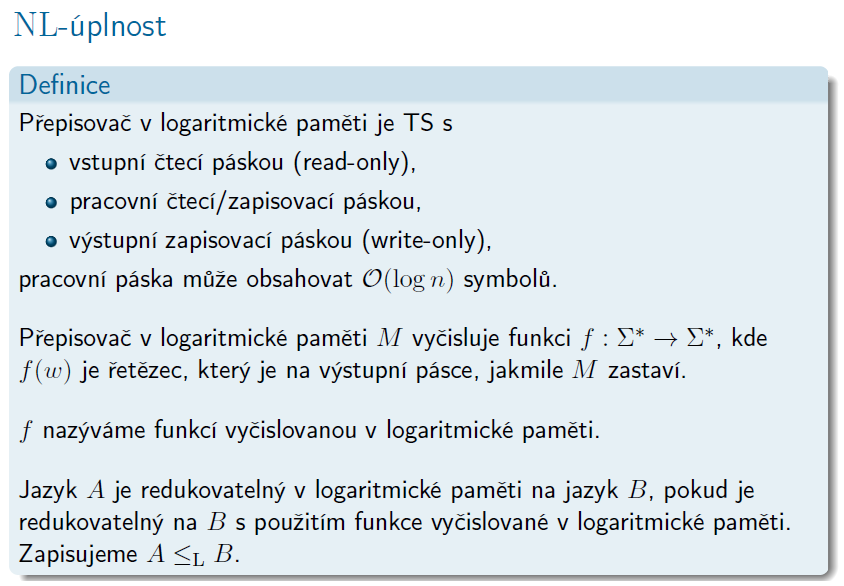
\includegraphics[width=13cm]{img/prepisovac}
		\end{figure}

		\begin{figure}[!h]
		\centering
		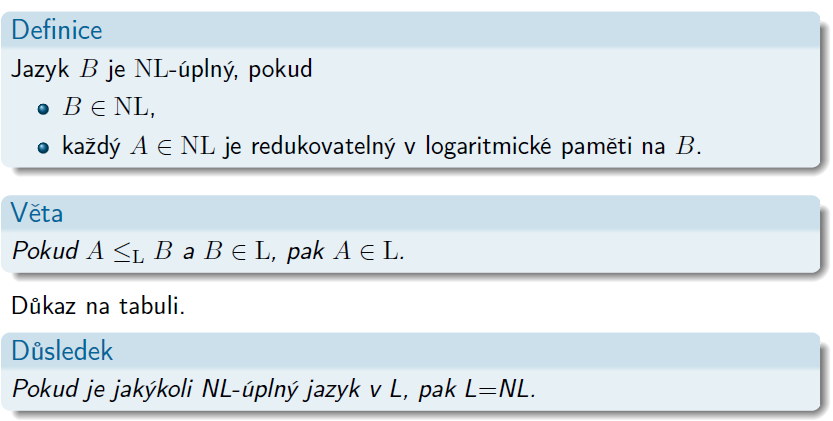
\includegraphics[width=13cm]{img/NLuplny}
		\end{figure}


%============================================================================
%                                                                            ČTVRTÝ ODSTAVEC
%============================================================================

\section{Čtvrtý odstavec}

Výroková logika: jazyk, formule, pravdivostní ohodnocení, tautologie, tabulková metoda, sémantické vyplývání,
normální formy formulí, úplné systémy spojek. Axiomatický systém výrokové logiky, syntaktické vyplývání. Věta
o dedukci. Věty o korektnosti a úplnosti výrokové logiky. Predikátová logika: jazyk, termy a formule, struktury
pro jazyk, ohodnocení termů a formulí. Axiomatický systém predikátové logiky, syntaktické vyplývání. Věty o
korektnosti a úplnosti predikátové logiky. Neklasické logiky, fuzzy logika. Základy logického programování, úvod
do Prologu.


	\subsection{Výroková Logika}

		\subsubsection{jazyk}
			\begin{figure}[!h]
			\centering
			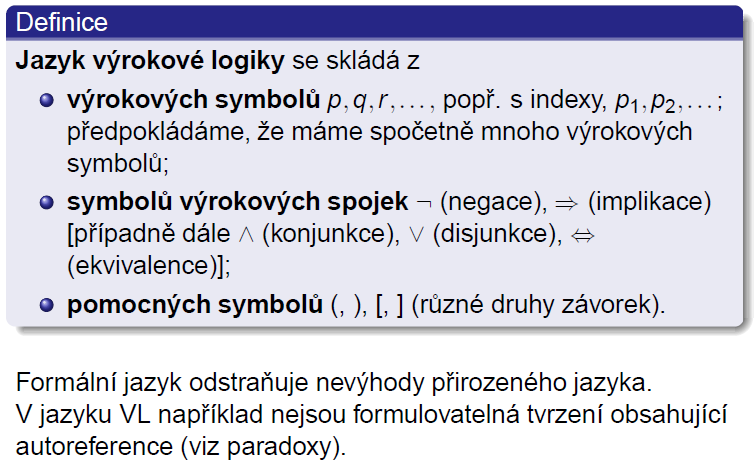
\includegraphics[width=13cm]{img/jazykVL}
			\end{figure}

			\begin{figure}[!h]
			\centering
			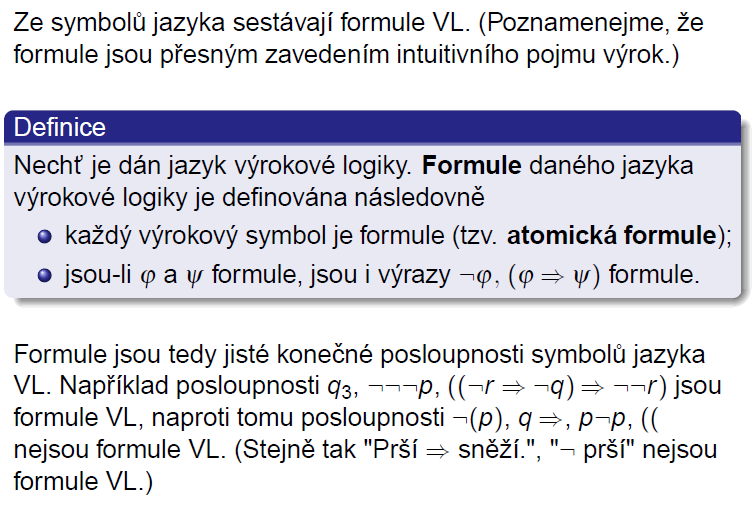
\includegraphics[width=13cm]{img/formuleVL}
			\end{figure}
 		\newpage
		\subsubsection{pravdivostní ohodnocení}

			\begin{figure}[!h]
			\centering
			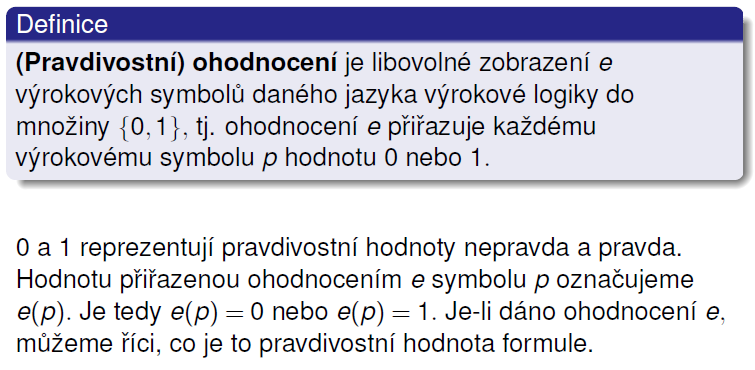
\includegraphics[width=13cm]{img/pravdivostniOhodnoceniVL}
			\end{figure}

			\begin{figure}[!h]
			\centering
			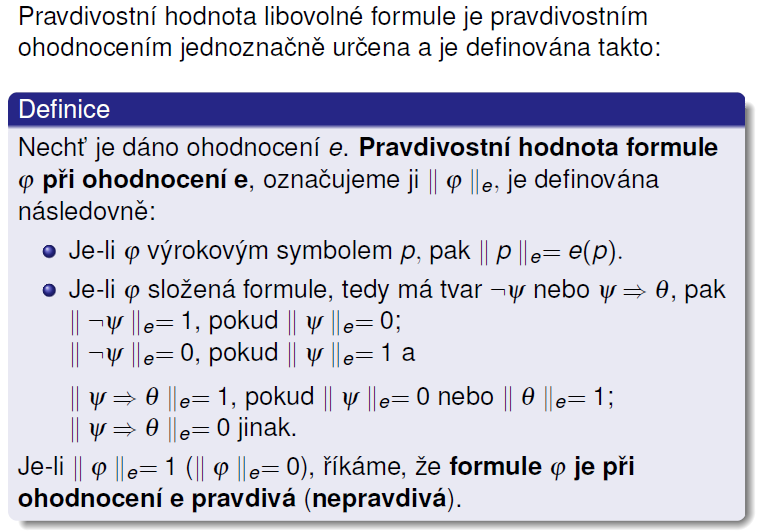
\includegraphics[width=13cm]{img/ohodnoceniFormule}
			\end{figure}

		\newpage
		\subsubsection{tautologie}

		\begin{figure}[!h]
			\centering
			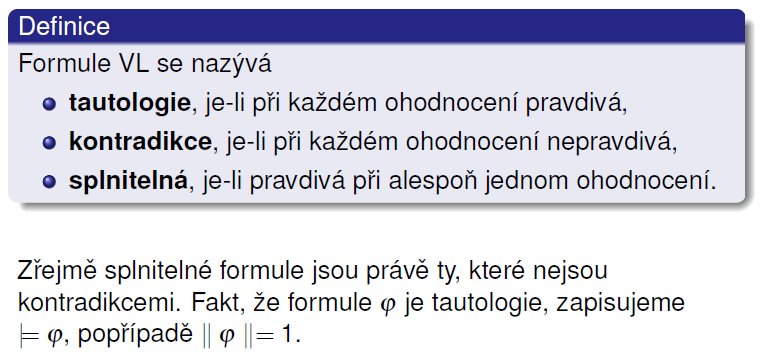
\includegraphics[width=13cm]{img/tautologie}
			\end{figure}

		\subsubsection{tabulková metoda}
			\begin{figure}[!h]
			\centering
			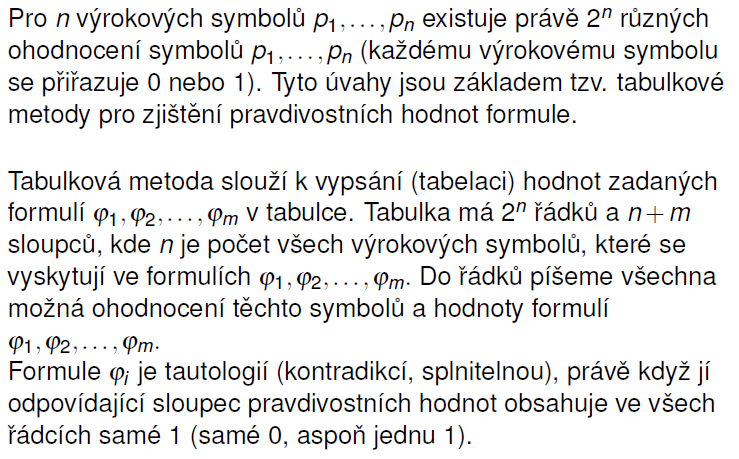
\includegraphics[width=13cm]{img/tabulkovaMetoda}
			\end{figure}

		\newpage
		\subsubsection{sémantické vyplývání}

			\begin{figure}[!h]
			\centering
			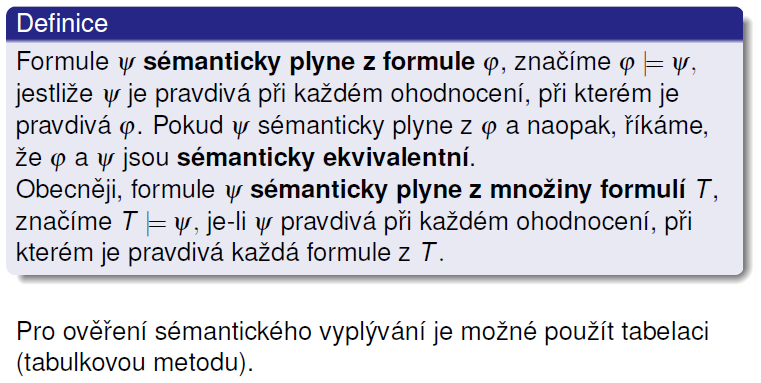
\includegraphics[width=13cm]{img/semantickeVyplyvani}
			\end{figure}

		\subsubsection{normální formy formulí}

			\begin{figure}[!h]
			\centering
			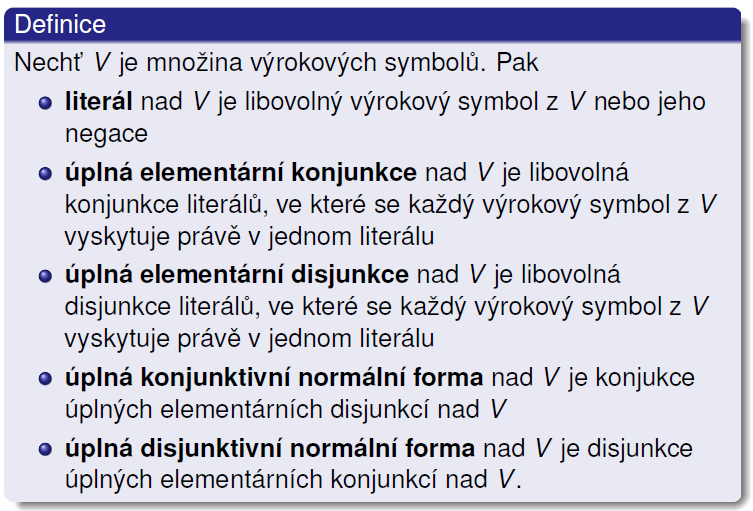
\includegraphics[width=13cm]{img/UKNF}
			\end{figure}

			\begin{figure}[!h]
			\centering
			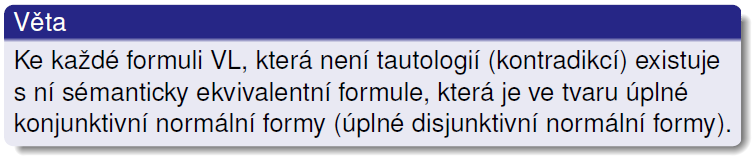
\includegraphics[width=13cm]{img/vetaUKNF}
			\end{figure}

			\begin{figure}[!h]
			\centering
			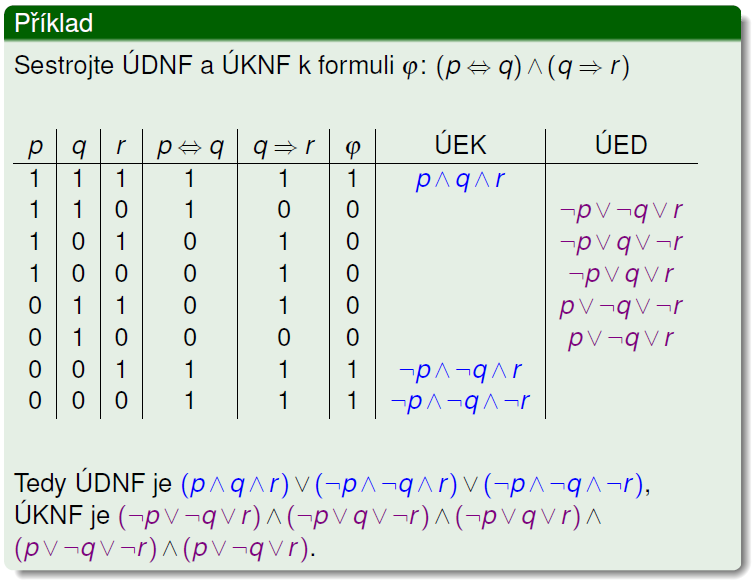
\includegraphics[width=13cm]{img/prikladUKNF}
			\end{figure}


		\subsubsection{úplné systémy spojek}

			\begin{figure}[H]
			\centering
			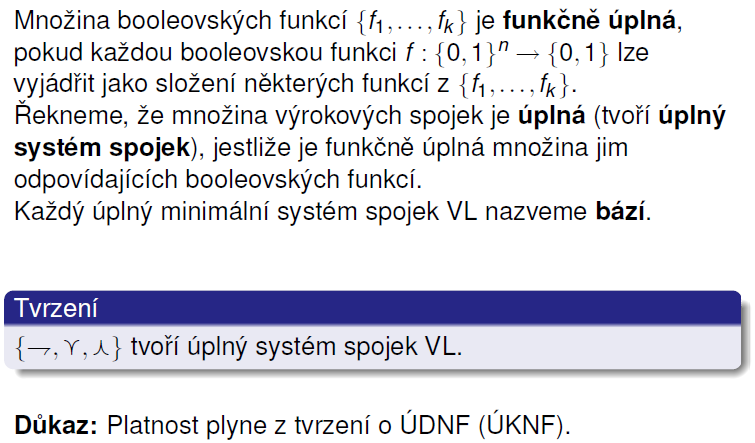
\includegraphics[width=13cm]{img/uplneSystemySpojek}
			\end{figure}

			\begin{figure}[H]
			\centering
			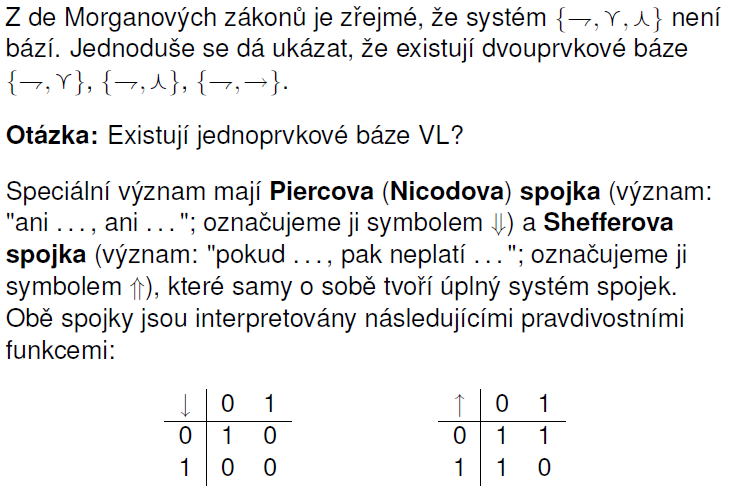
\includegraphics[width=13cm]{img/uplneSystemySpojek2}
			\end{figure}

			Existují pouze 2 jednoprvkové báze (Sheffer a Nicod)

		\subsubsection{axiomatický systém výrokové logiky}

			\begin{figure}[H]
			\centering
			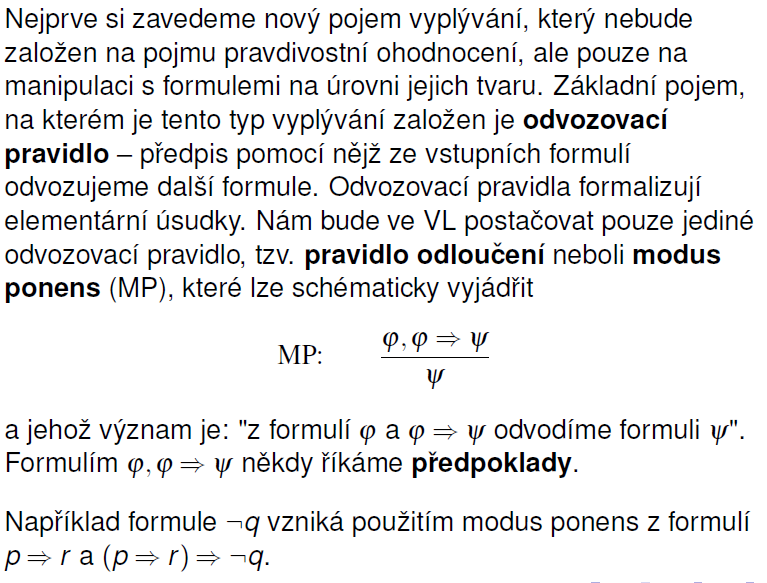
\includegraphics[width=12cm]{img/MP}
			\end{figure}

			\begin{figure}[H]
			\centering
			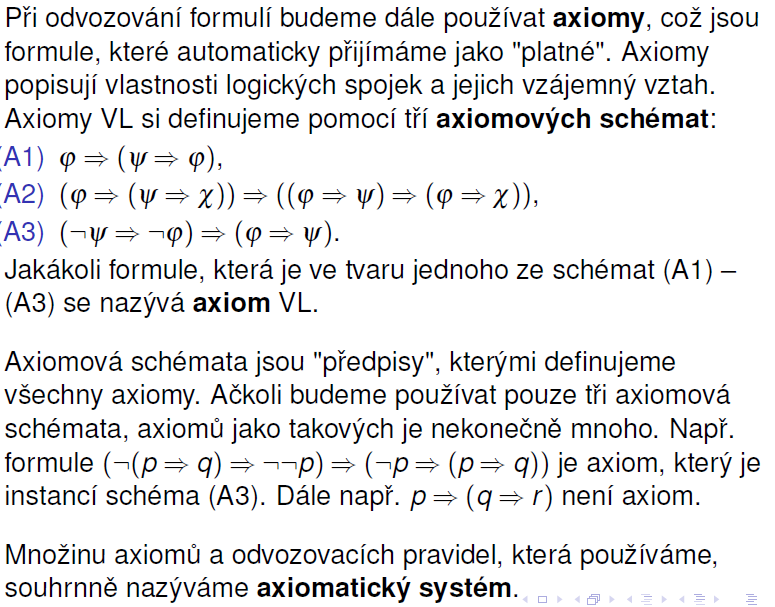
\includegraphics[width=12cm]{img/axiomy}
			\end{figure}

		\subsubsection{syntaktické výplývání}

			\begin{figure}[H]
			\centering
			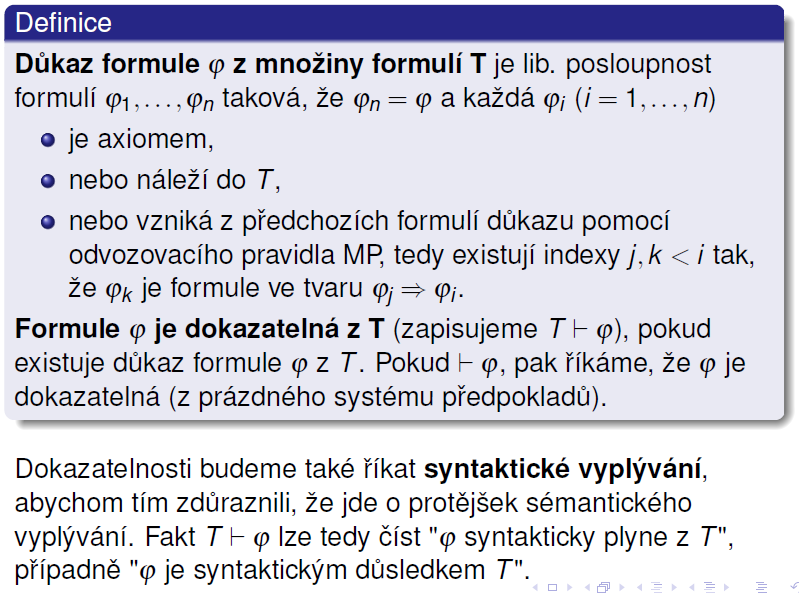
\includegraphics[width=12cm]{img/dukaz}
			\end{figure}

		\subsubsection{Věta o dedukci}

			\begin{figure}[H]
			\centering
			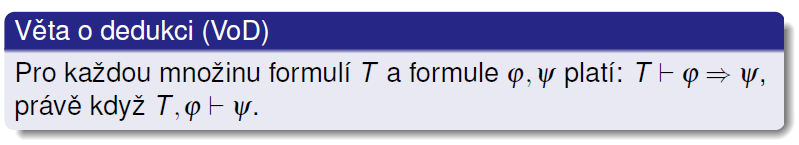
\includegraphics[width=13cm]{img/VoD}
			\end{figure}

			\begin{figure}[H]
			\centering
			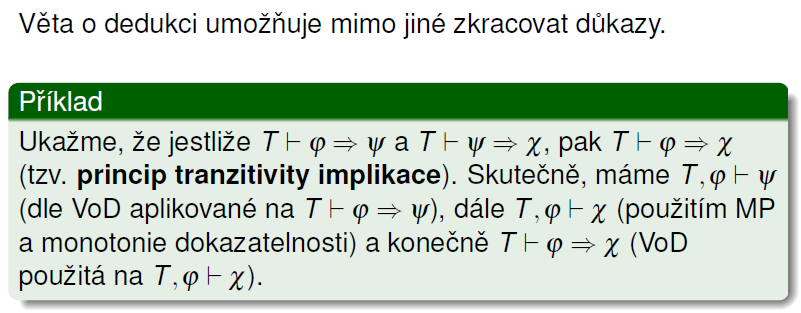
\includegraphics[width=13cm]{img/VoDpriklad}
			\end{figure}

		\subsubsection{Věty o korektnosti a úplnosti výrokové logiky}

			\begin{figure}[H]
			\centering
			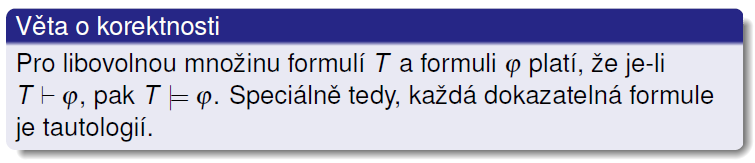
\includegraphics[width=13cm]{img/VoK}
			\end{figure}

			\begin{figure}[H]
			\centering
			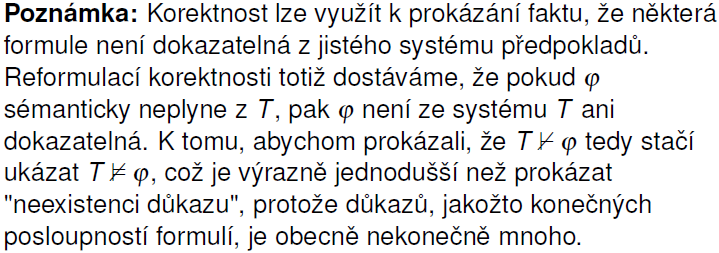
\includegraphics[width=13cm]{img/VoKpoznamka}
			\end{figure}

			\begin{figure}[H]
			\centering
			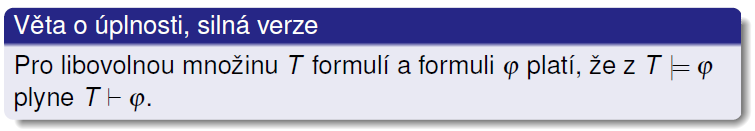
\includegraphics[width=13cm]{img/VoU}
			\end{figure}

	\subsection{Predikátová logika}

		\subsubsection{jazyk}

			\begin{figure}[H]
			\centering
			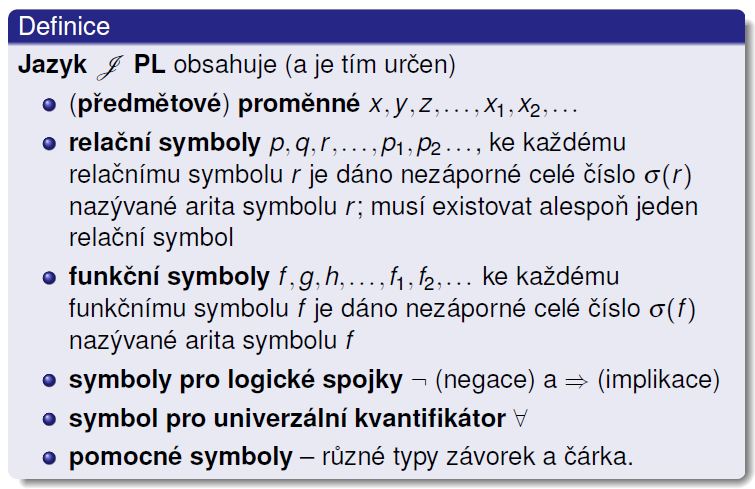
\includegraphics[width=13cm]{img/JazykPL}
			\end{figure}

			\begin{figure}[H]
			\centering
			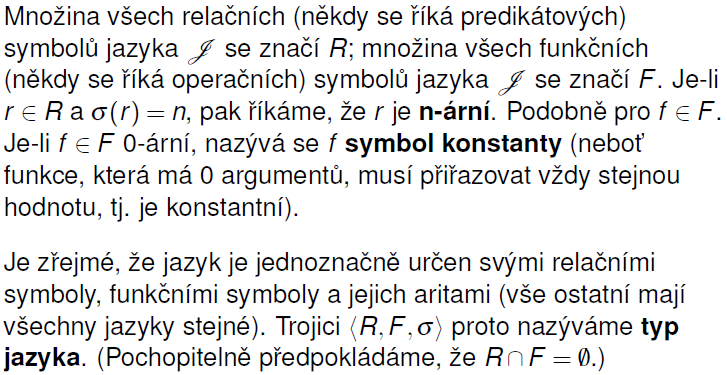
\includegraphics[width=13cm]{img/JazykPL2}
			\end{figure}

		\subsubsection{termy a formule}

			\begin{figure}[H]
			\centering
			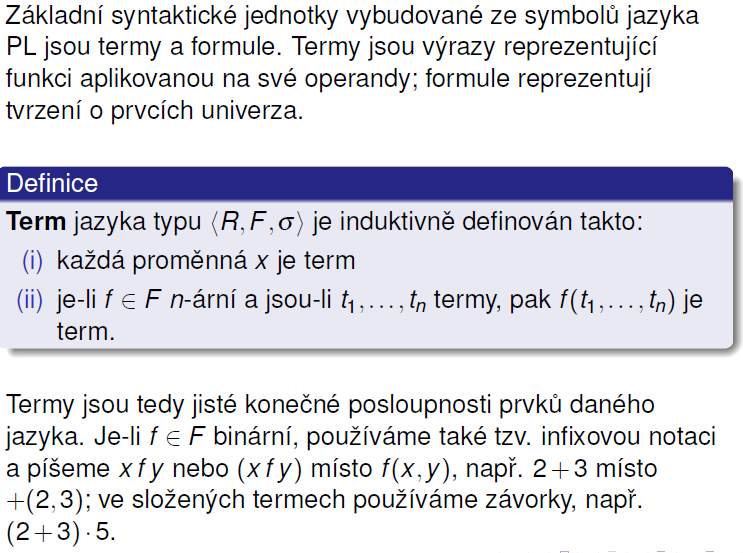
\includegraphics[width=13cm]{img/termy}
			\end{figure}

			\begin{figure}[H]
			\centering
			\includegraphics[width=13cm]{img/formulePL}
			\end{figure}

		\subsubsection{struktury pro jazyk}

			\begin{figure}[H]
			\centering
			\includegraphics[width=13cm]{img/stukturaProJazyk}
			\end{figure}

			\begin{figure}[H]
			\centering
			\includegraphics[width=13cm]{img/strukturaProJazyk}
			\end{figure}

		\subsubsection{ohodnocení termu a formulí}

			\begin{figure}[H]
			\centering
			\includegraphics[width=13cm]{img/ohodnoceniPL}
			\end{figure}

			\begin{figure}[H]
			\centering
			\includegraphics[width=13cm]{img/mOhodnoceni}
			\end{figure}

			\begin{figure}[H]
			\centering
			\includegraphics[width=13cm]{img/ohodnoceniFormuliPL}
			\end{figure}

		\subsubsection{axiomatický systém predikátové logiky}

			\begin{figure}[H]
			\centering
			\includegraphics[width=13cm]{img/axiomyPL}
			\end{figure}

		\subsubsection{syntaktické vyplývání}

			\begin{figure}[H]
			\centering
			\includegraphics[width=13cm]{img/semantickeVyplyvaniPL}
			\end{figure}

			\begin{figure}[H]
			\centering
			\includegraphics[width=13cm]{img/syntaktickeVyplyvaniPL}
			\end{figure}

			Formule je dokazatelná z T = formule syntakticky plyne z T.


		\subsubsection{věty o korektnosti a úplnosti predikátové logiky}

			\begin{figure}[H]
			\centering
			\includegraphics[width=13cm]{img/VoKPL}
			\end{figure}

			\begin{figure}[H]
			\centering
			\includegraphics[width=13cm]{img/VoUPL}
			\end{figure}

	\subsection{Neklasické logiky}
		\begin{itemize}
			\item Modální logika (založena na pojmu \uv{možný svět}, spojky:\textit{ je možné že, je nutné že})
			\item Temporální logika (logika času - pravdivost tvrzení závisí na čase)
			\item Epistemická logika (logika znalostí, spojky: \textit{ví se že, věří se že})
			\item Fuzzy logika
		\end{itemize}

		\subsubsection{fuzzy logika}

			\begin{figure}[H]
			\centering
			\includegraphics[width=13cm]{img/fuzzy1}
			\end{figure}

			\begin{figure}[H]
			\centering
			\includegraphics[width=13cm]{img/fuzzy2}
			\end{figure}

			\begin{figure}[H]
			\centering
			\includegraphics[width=13cm]{img/fuzzy3}
			\end{figure}

			\begin{figure}[H]
			\centering
			\includegraphics[width=13cm]{img/fuzzy4}
			\end{figure}


	\subsection{Základy logického programování, úvod do Prologu}

			\begin{figure}[H]
			\centering
			\includegraphics[width=13cm]{img/prolog1}
			\end{figure}

			\begin{figure}[H]
			\centering
			\includegraphics[width=13cm]{img/prolog2}
			\end{figure}

			\begin{figure}[H]
			\centering
			\includegraphics[width=13cm]{img/prolog3}
			\end{figure}

			\begin{figure}[H]
			\centering
			\includegraphics[width=13cm]{img/prolog4}
			\end{figure}

			\begin{figure}[H]
			\centering
			\includegraphics[width=13cm]{img/prolog5}
			\end{figure}

			\begin{figure}[H]
			\centering
			\includegraphics[width=13cm]{img/prolog6}
			\end{figure}

			\begin{figure}[H]
			\centering
			\includegraphics[width=13cm]{img/prolog7}
			\end{figure}

			\begin{figure}[H]
			\centering
			\includegraphics[width=13cm]{img/prolog8}
			\end{figure}

			\begin{figure}[H]
			\centering
			\includegraphics[width=13cm]{img/prolog9}
			\end{figure}

	Zbytek prologu už je nechutně hnusnej a radši chcípnu než abych se to zas učil.


\end{document}
